\documentclass{article}

\usepackage[utf8]{inputenc}
\usepackage[T1]{fontenc}
\usepackage{geometry}
\usepackage{xcolor}
\usepackage{graphicx}
\usepackage{subcaption}
\usepackage{verbatim}
\usepackage{amsmath,amssymb}
\usepackage{amstext}
\usepackage{amsthm}
\usepackage{steinmetz}
\usepackage{stackrel}
\usepackage{mathtools}
\geometry{a4paper}

\usepackage[french,italian]{babel}
\frenchspacing

\counterwithin{figure}{section}
\counterwithin{table}{section}

\title{Dispensa del laboratorio di elettronica (LOEFM)}
\author{Lorenzo Ramella, Alessandro Matteo Rossi, Marco Tambini}
\date{AA 2020-2021}

\begin{document}
\maketitle

\begin{figure}[h]
  \centering
  %\captionsetup{justification=centering,margin=2cm}
  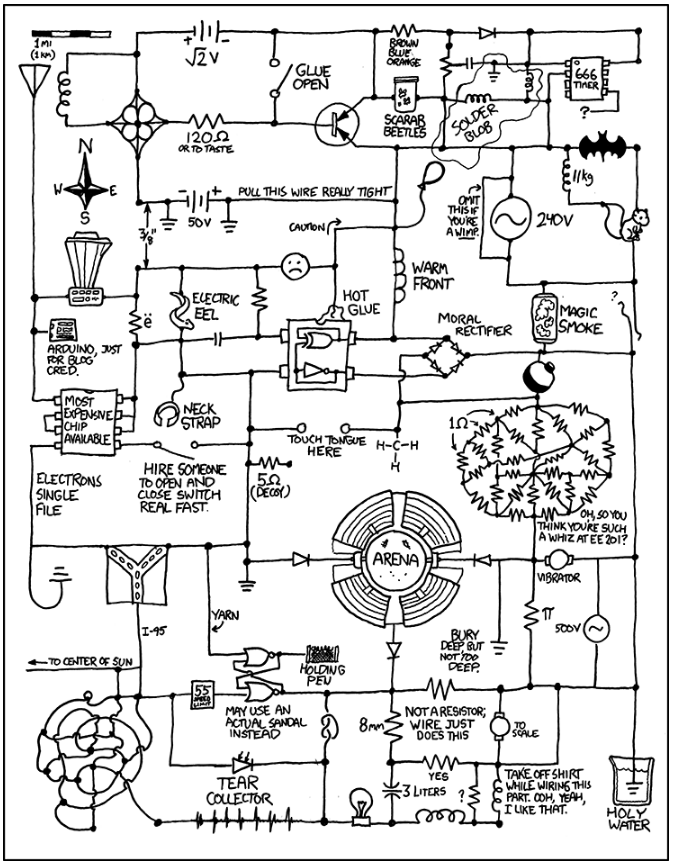
\includegraphics[scale=0.6]{IM_relevant_xkcd}
  \caption*{Relevant xkcd}
\end{figure}

\clearpage

\begin{abstract}

Le lezioni del prof. Stefano Riboldi relative al laboratorio di elettronica del secondo anno, "sbobinate".

\end{abstract}
\tableofcontents

\clearpage








\section{Richiami alle nozioni di base}

\subsection{Generatori}

\begin{figure}[h]
  \centering
  %\captionsetup{justification=centering,margin=2cm}
  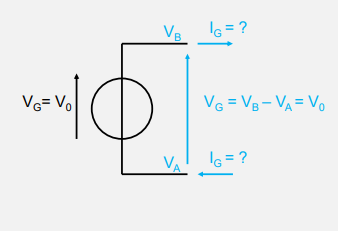
\includegraphics[scale=0.6]{IM_generatori_tensione}
  \caption{Schizzo di un generatore ideale di tensione}
  \label{Schema_generatori_tensione}
\end{figure}

Un \textit{generatore ideale di tensione} è un dipolo a due terminali il quale matematicamente definisce una relazione tra i potenziali ai due capi del generatore, ovvero impone la differenza di potenziale ad un valore fisso. 

\vspace{1mm}

In un dipolo è possibile definire una differenza di potenziale $V$ e una corrente $I$. In un generatore di tensione la prima è imposta dal generatore stesso, mentre la seconda dipende dal circuito esterno. Nel caso schematizzato in figura \ref{Schema_generatori_tensione}, essendo il circuito aperto, $I_G = 0$.

\vspace{1mm}

La potenza generata è pari a 

\[P_G = V_G \cdot I_G\]

Si noti che, usando la convenzione dei generatori, la potenza è \textit{generata} (quindi positiva) se la corrente è uscente dal lato della tensione positiva, essendo in questa convenzione il verso della tensione concorde con il verso della corrente. Quando si lavora sugli utilizzatori si usa la convenzione opposta. Un esempio di generatore di tensione può essere una classica pila.

\begin{figure}[h]
  \centering
  %\captionsetup{justification=centering,margin=2cm}
  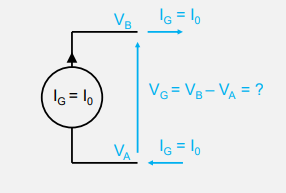
\includegraphics[scale=0.6]{IM_generatori_corrente}
  \caption{Schizzo di un generatore ideale di corrente}
  \label{Schema_generatori_corrente}
\end{figure}

Nel caso di un \textit{generatore di corrente}, invece, il generatore impone la corrente, mentre la tensione dipende dal circuito esterno.

La potenza generata, con la convenzione dei generatori, è sempre 

\[P_G = V_G \cdot I_G\]

Questi generatori sono meno comuni dei generatori di tensione.

\clearpage






\subsection{Resistori}

\begin{figure}[h]
  \centering
  %\captionsetup{justification=centering,margin=2cm}
  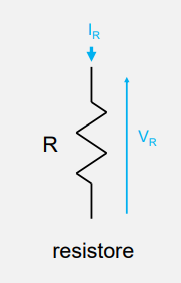
\includegraphics[scale=0.7]{IM_resistore}
  \caption{Schizzo di un resistore}
  \label{Schema_resistore}
\end{figure}

Il \textit{resistore} (o \textit{resistenza}) è il primo esempio di elemento \textit{passivo}, o \textit{di carico}, a cui è possibile collegare un generatore. È un dipolo, quindi si può definire ai suoi capi una differenza di potenziale $V_R$ ed una corrente $I_R$. Si noti, come schematizzato in figura \ref{Schema_resistore}, che il verso della corrente è discorde con il verso della tensione. Questa è la cosiddetta convenzione degli utilizzatori, opposta a quella dei generatori.

\vspace{3mm}

\textbf{Legge di Ohm:} all'interno di un resistore esiste una precisa relazione tra le grandezze $V_R$ e $I_R$:

\[\frac{V_R}{I_R} = \textit{ costante } = R [\Omega] = \frac{1}{G [\textrm S]}\]

$R$ è la \textit{resistenza} e si misura in ohm ($\Omega$). $G$ è la \textit{conduttanza} e si misura in siemens (S). La legge di Ohm è spesso scritta nella forma

\begin{equation}
V = R \cdot I
\label{Ohm}
\end{equation}

Poiché $R$ non è un parametro che dipende dal tempo, la legge di Ohm evolve nel tempo semplicemente come

\[V_R (t) = I_R (t) \cdot R\]

La potenza, questa volta \textit{dissipata}, è 

\[P_R (t) = V_R (t) \cdot I_R (t) \quad \textrm{oppure} \quad P_R (t) = V_R^2 (t) / R\]

spesso scritta nella forma della \textbf{legge di Joule:}

\begin{equation}
P_R (t) = I_R^2 (t) \cdot R
\label{Joule}
\end{equation}

\textbf{Nota importante:} dalla legge di Joule si evince che, facendo passare corrente in un resistore, questo dissipa energia, quindi si scalda. In laboratorio è importante prestare la massima attenzione per evitare ustioni.

\newpage








\subsection{Condensatori}

\begin{figure}[h!]
  \centering
  %\captionsetup{justification=centering,margin=2cm}
  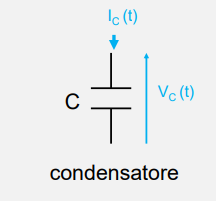
\includegraphics[scale=0.65]{IM_condensatore}
  \caption{Schizzo di un condensatore}
  \label{Schema_condensatore}
\end{figure}

Un \textit{condensatore} immagazzina al suo interno una carica $Q$, misurata in coulomb (C). Questa è l'integrale della corrente che attraversa il condensatore nel tempo.

In un condensatore esiste una relazione tra la carica in esso immagazzinata e la differenza di potenziale ai suoi capi:

\[\frac{Q_C (t)}{V_C (t)} = C [\textrm F]\]

$C$ è la \textit{capacità}, e si misura in farad (F), ed è una costante positiva.

\[I_C (t) = \frac{\textrm d Q_C (t)}{\textrm d t} = C \frac{\textrm d V_C (t)}{\textrm d t}\]

Un condensatore è in grado di immagazzinare un'energia

\[E_C (t) = \frac{1}{2} Q_C (t) V_C (t) = \frac{1}{2} C V_C^2 (t)\]










\subsection{Induttori}

\begin{figure}[h]
  \centering
  %\captionsetup{justification=centering,margin=2cm}
  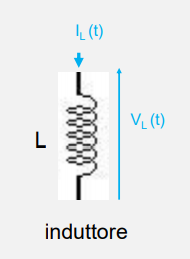
\includegraphics[scale=0.6]{IM_induttore}
  \caption{Schizzo di un induttore}
  \label{Schema_induttore}
\end{figure}

L'\textit{induttore}, meno diffuso del condensatore, ne è l'\textit{elemento duale}. Detto $\Phi$ il flusso del campo magnetico, misurato in weber (Wb), si ha che 

\[\frac{\Phi _L (t)}{I_L (t)} = \textit{ costante positiva } = L \]

$L$ è detta \textit{induttanza} e si misura in henry [H]. 

\[V_L = \frac{\textrm d \Phi _L (t)}{\textrm d t} = L \frac{\textrm d I _L (t)}{\textrm d t}\]

Mentre nel condensatore era la corrente ad essere proporzionale alla derivata della tensione rispetto al tempo, qui è la tensione ad essere proporzionale alla derivata della corrente rispetto al tempo. L'energia immagazzinata è

\[E_L (t) = \frac{1}{2} \Phi _L (t) I_L (t) = \frac{1}{2} L I_L^2 (t)\]

L'induttore, pur essendo analogo al condensatore, ha dei comportamenti controintuitivi. Per esempio, cortocircuitando un condensatore si disperde tutta l'energia in esso immagazzinata, mentre per mantenere l'energia immagazzinata bisogna isolarlo. 

\vspace{3mm}

Nell'induttore l'energia immagazzinata dipende dalla corrente: affinché si mantenga l'energia immagazzinata in un induttore, quindi, serve che la derivata delle corrente rispetto al tempo sia nulla, ovvero che la differenza di potenziale ai due poli dell'induttore sia nulla. Quindi, per mantenere l'energia immagazzinata, bisogna cortocircuitare l'induttore.









\subsection{Circuiti RC nel tempo}

\begin{figure}[h]
  \centering
  %\captionsetup{justification=centering,margin=2cm}
  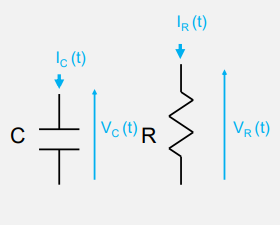
\includegraphics[scale=0.7]{IM_circuito_RC}
  \caption{Schizzo di un circuito RC ($t<0$)}
  \label{Schema_circuito_RC}
\end{figure}

Un \textit{circuito RC} è un sistema a 4 gradi di libertà (2 tensioni e 2 correnti), essendo costituito da 2 dipoli. Nel caso schematizzato in figura \ref{Schema_circuito_RC}, per t<0 le condizioni al contorno sono:

\begin{itemize}
  \item $I_R (t) = 0$ (dipolo non connesso)
  \item $I_C (t) = 0$ (dipolo non connesso)
  \item $V_R (t) = 0$ (legge di Ohm)
  \item $V_C (t) = \frac{q_0}{C} = v_0$
\end{itemize}
\newpage
Chiudendo il circuito come illustrato in figura \ref{Schema_circuito_RC_chiuso} si ha che:

\begin{figure}[h]
  \centering
  %\captionsetup{justification=centering,margin=2cm}
  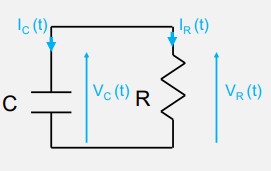
\includegraphics[scale=0.7]{IM_circuito_RC_chiuso}
  \caption{Schizzo di un circuito RC ($t>0$)}
  \label{Schema_circuito_RC_chiuso}
\end{figure}

\begin{itemize}
  \item $I_C (t) = - I_R (t)$ (dipoli in serie e frecce discordi)
  \item $V_C (t) = V_R (t)$ (dipoli in parallelo e frecce concordi)
  \item $\frac{\textrm d V_C (t)}{\textrm d t} = \frac{I_C (t)}{C} = - \frac{I_R (t)}{C} = -\frac{V_R (t)}{CR} = -\frac{V_C (t)}{CR}$
  \item $V_C (t) = V_R (t) = v_0 \cdot e^{-t/(CR)}$
  \item $I_C (t) = -I_R (t) = \frac{v_0}{R} \cdot e^{-t/(CR)}$
\end{itemize}

Dopo aver notato il fatto che la quantità $CR$ ha la dimensione dei secondi, la si può anche riscrivere come $\tau = CR$.








\subsection{Circuiti RL nel tempo}

\begin{figure}[h]
  \centering
  %\captionsetup{justification=centering,margin=2cm}
  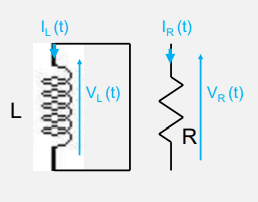
\includegraphics[scale=0.7]{IM_circuito_RL}
  \caption{Schizzo di un circuito RL (t<0)}
  \label{Schema_circuito_RL}
\end{figure}

Un \textit{circuito RL} è un sistema sempre a 4 gradi di libertà (2 tensioni e 2 correnti). Nel caso schematizzato in figura \ref{Schema_circuito_RL}, per $t<0$ le condizioni al contorno sono:

\begin{itemize}
  \item $I_R (t) = 0$ (dipolo non connesso)
  \item $V_R (t) = 0$ (legge di Ohm)
  \item $V_L (t) = 0$
  \item $I_L (t) = \frac{\phi _0}{L} = i_0$ (la corrente si mantiene perché l'induttore è in cortocircuito)
\end{itemize}
\newpage
Chiudendo il circuito come illustrato in figura \ref{Schema_circuito_RL_chiuso} si ha che:

\begin{figure}[h]
  \centering
  %\captionsetup{justification=centering,margin=2cm}
  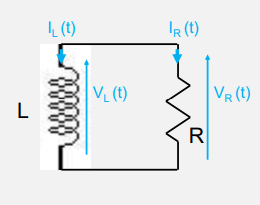
\includegraphics[scale=0.7]{IM_circuito_RL_chiuso}
  \caption{Schizzo di un circuito RL ($t>0$)}
  \label{Schema_circuito_RL_chiuso}
\end{figure}

\begin{itemize}
  \item $I_L (t) = - I_R (t)$ (dipoli in serie e frecce discordi)
  \item $V_L (t) = V_R (t)$ (dipoli in parallelo e frecce concordi)
  \item $\frac{\textrm d I_L (t)}{\textrm d t} = \frac{V_L (t)}{L} = \frac{V_R (t)}{L} = -I_R (t) \frac{R}{L} = -I_L (t) \frac{R}{L}$
  \item $I_L (t) = -I_R (t) = i_0 \cdot e^{-t/\tau}$
  \item $V_L (t) = V_R (t) = i_0 \cdot R \cdot e^{-t/\tau}$
\end{itemize}

Dove $\tau = L/R$.











\newpage

\section{Leggi circuitali e concetti fondamentali}

\subsection{Leggi di Kirchhoff}

Dato un circuito costituido da dipoli, definiamo:

\begin{figure}[h]
  \centering
  %\captionsetup{justification=centering,margin=2cm}
  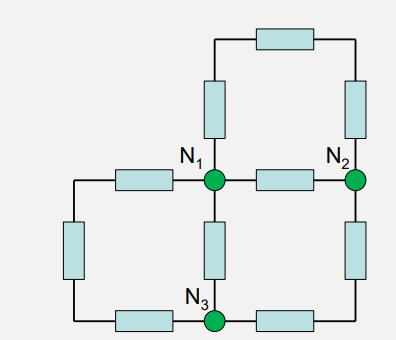
\includegraphics[scale=0.4]{IM_kirchhoff_nodi}
  \caption{Schizzo di un circuito di dipoli. In verde i nodi}
  \label{Schema_nodi}
\end{figure}

\textit{Nodi} i punti di contatto tra 3 o più dipoli (figura \ref{Schema_nodi});

\begin{figure}[h]
  \centering
  %\captionsetup{justification=centering,margin=2cm}
  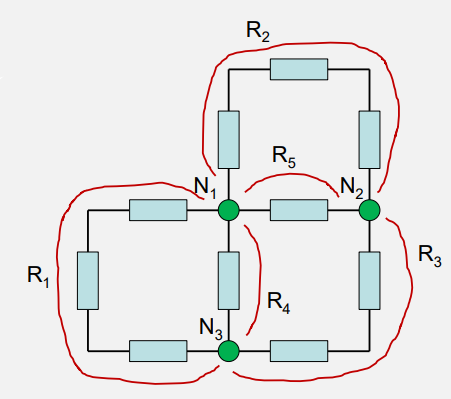
\includegraphics[scale=0.4]{IM_kirchhoff_rami}
  \caption{Schizzo di un circuito di dipoli. In rosso i rami}
  \label{Schema_rami}
\end{figure}

\textit{Rami} i percorsi compresi tra due nodi (figura \ref{Schema_rami});

\begin{figure}[h]
  \centering
  %\captionsetup{justification=centering,margin=2cm}
  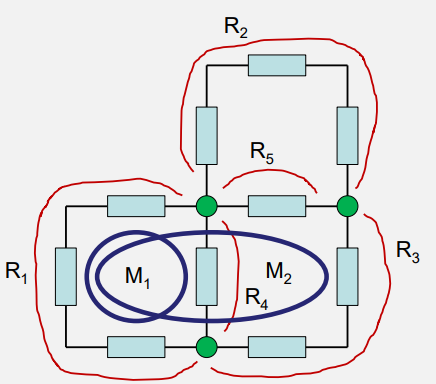
\includegraphics[scale=0.4]{IM_kirchhoff_maglie}
  \caption{Schizzo di un circuito di dipoli. In blu le maglie}
  \label{Schema_maglie}
\end{figure}

\textit{Maglie} insiemi chiusi di rami (figura \ref{Schema_maglie});
\newpage
Partendo da queste definizioni, introduciamo le due \textit{leggi di Kirchhoff}:

\vspace{3mm}

\textbf{La legge delle correnti (KCL):} La somma algebrica delle correnti nei rami afferenti a ciascun nodo è nulla.

\begin{equation}
\sum I_n = 0
\label{KCL}
\end{equation}

In altre parole: a ciascun nodo, la somma delle correnti  entranti è pari alla somma delle correnti uscenti.

\vspace{3mm}

\textbf{La legge delle tensioni (KVL):} La somma algebrica delle tensioni sui rami di ciascuna maglia è nulla.

\begin{equation}
\sum V_n = 0
\label{KVL}
\end{equation}

In altre parole: la somma algebrica delle differenze di potenziale su ogni percorso che unisce due medesimi punti è costante.







\subsection{Circuiti partitori di tensione e corrente}

\begin{figure}[h]
  \centering
  %\captionsetup{justification=centering,margin=2cm}
  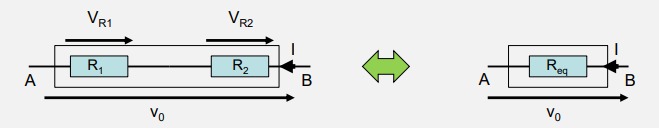
\includegraphics[scale=0.7]{IM_circuiti_partitori}
  \caption{Schizzo di un sistema di due dipoli in serie (partitore di tensione)}
  \label{Schema_dipoli_serie}
\end{figure}

Due dipoli sono detti \textit{in serie} se (e solo se) condividono la stessa corrente. Dalle equazioni \ref{Ohm} e \ref{KVL} sappiamo rispettivamente che

\[V_{R1} = I \cdot R_1 \quad \textrm{e} \quad V_{R2} = I \cdot R_2\]

\[V_{R1} + V_{R2} = V_0\]

quindi

\[V_0 = I \cdot (R_1 + R_2) \Rightarrow I = \frac{V_0}{R_1 + R_2} = \frac{V_0}{R_{eq}}\]

\[R_{eq} = R_1 + R_2\]

Se ho due o più resistenze collegate in serie, esse equivalgono ad un unico resistore la cui resistenza equivalente è pari alla somma delle singole resistenze.

\vspace{3mm}

Se si volesse ora trovare il valore di $V_{R1}$ basta pensare che

\[V_{R1} = I \cdot R_1 = V_0 \frac{R_1}{R_{eq}}\]

\begin{figure}[h]
  \centering
  %\captionsetup{justification=centering,margin=2cm}
  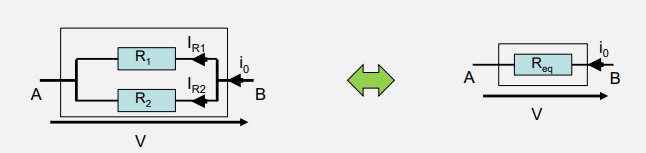
\includegraphics[scale=0.7]{IM_circuiti_partitori_bis}
  \caption{Schizzo di un sistema di due dipoli in parallelo (partitore di corrente)}
  \label{Schema_dipoli_parallelo}
\end{figure}

Due dipoli sono detti \textit{in parallelo} se (e solo se) condividono la stessa tensione. Dalle equazioni \ref{Ohm} e \ref{KCL} sappiamo rispettivamente che

\[V = I_1 \cdot R_1 \quad \textrm{e} \quad V = I_2 \cdot R_2\]

\[I_{R1} + I_{R2} = I_0\]

quindi

\[I_0 =\frac{V}{R_1} + \frac{V}{R_2} \Rightarrow I_0 = V \left( \frac{1}{R_1}+ \frac{1}{R_2} \right) = V \left( \frac{R_1 + R_2}{R_1 R_2} \right)\]

\[R_{eq} = \frac{R_1 R_2}{R_1 + R_2} \quad \textrm{oppure} \quad \frac{1}{R_{eq}}=\left( \frac{1}{R_1}+ \frac{1}{R_2} \right)\]

Se ho due o più resistenze collegate in parallelo, esse equivalgono ad un unico resistore la cui resistenza equivalente è pari alla somma armonica delle singole resistenze.

\vspace{3mm}

\textbf{Nota importante:} d'ora in avanti si userà il simbolo $//$ per indicare la somma armonica tra due o più quantità.

\[\displaystyle{\left(\frac{1}{R_1}+\frac{1}{R_2}\right)^{-1}:= R_1//R_2}\]

\vspace{3mm}

Se si volesse ora trovare il valore di $I_{R1}$ basta pensare che

\[I_{R1} = \frac{V}{R_1} = I_0 \frac{R_{eq}}{R_1} = I_0 \frac{R_2}{R_1 + R_2}\]

\clearpage










\subsection{Generatori reali}

\begin{figure}[h]
  \centering
  %\captionsetup{justification=centering,margin=2cm}
  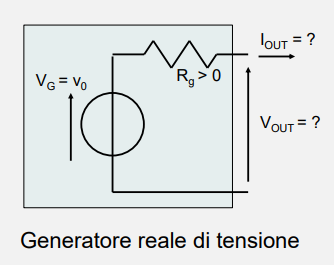
\includegraphics[scale=0.5]{IM_generatori_reali_tensione}
  \caption{Schizzo di un generatore reale di tensione}
  \label{Schema_generatore_reale_tensione}
\end{figure}

In un \textit{generatore reale}, si distingue la differenza di potenziale ai capi del generatore $V_G$ dalla differenza di potenziale ai capi del sistema a cui il generatore è collegato:

\[V_{OUT} = V_G - V_R\]

dove $V_R$ è la \textit{caduta di tensione} ai capi del resistore $R_g$ dovuta alla corrente che scorre all'esterno del circuito. Quindi:

\begin{itemize}
  \item $V_{OUT}$ dipende anche dal circuito esterno
  \item $I_{OUT}$ dipende anche dal circuito esterno
  \item $P_{OUT}$ (generata) $= V_{OUT} \cdot I_{OUT}$
\end{itemize}

\begin{figure}[h]
  \centering
  %\captionsetup{justification=centering,margin=2cm}
  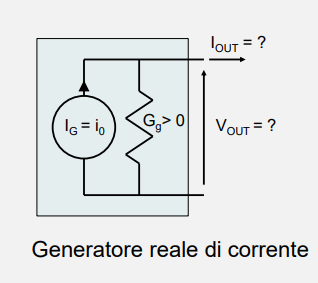
\includegraphics[scale=0.5]{IM_generatori_reali_corrente}
  \caption{Schizzo di un generatore reale di corrente}
  \label{Schema_generatore_reale_corrente}
\end{figure}

Con un discorso analogo a quello del caso precedente ricaviamo che

\begin{itemize}
  \item $I_{OUT}$ dipende anche dal circuito esterno
  \item $V_{OUT}$ dipende anche dal circuito esterno
  \item $P_{OUT}$ (generata) $= V_{OUT} \cdot I_{OUT}$
\end{itemize}

\clearpage












\subsection{Circuiti equivalenti di Thevenin e di Norton}

\begin{figure}[h]
  \centering
  %\captionsetup{justification=centering,margin=2cm}
  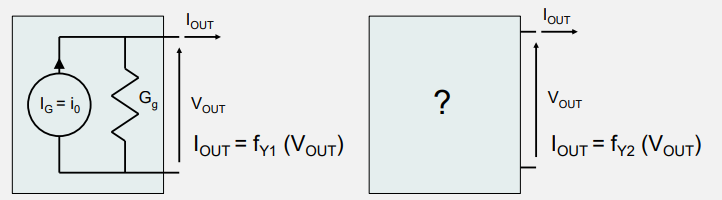
\includegraphics[scale=0.7]{IM_Thevenin_Norton}
  \caption{Il dipolo ignoto}
  \label{Schema_Thevenin_Norton}
\end{figure}

Si immagini di prendere il dipolo rappresentato in figura \ref{Schema_Thevenin_Norton}. Come caratterizzarlo senza ``aprire'' la scatola?

\vspace{1mm}

Poiché le uniche due grandezze misurabili sono la tensione e la corrente, l'unico strumento che si ha a disposizione è la \textit{curva caratteristica} $I-V$:
\[I_{OUT} = f_Y(V_{OUT}) \quad \textrm{oppure} \quad V_{OUT} = f_Z(I_{OUT})\]
Due dipoli sono \textit{equivalenti} se e solo se hanno la stessa curva caratteristica.

\vspace{1mm}

Se le relazioni sono lineari basta determinarne 2 punti. Come nell'esempio mostrato in figura \ref{Schema_Thevenin_Norton_bis}

\begin{figure}[h]
  \centering
  %\captionsetup{justification=centering,margin=2cm}
  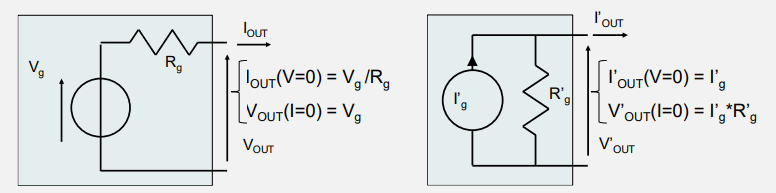
\includegraphics[scale=0.7]{IM_Thevenin_Norton_bis}
  \caption{Esempio di due dipoli di cui determinare l'equivalenza}
  \label{Schema_Thevenin_Norton_bis}
\end{figure}

Imponendo $I_{OUT} (0) = I'_{OUT} (0)$ e $V_{OUT} (0) = V'_{OUT} (0)$ si trovano le relazioni

\[R_g = R'_g\]

\[V_g = I'_g \cdot R'_g\]

Ne segue che i due circuiti (quando soddisfano queste due condizioni), pur essendo circuiti diversi, sono equivalenti.

\vspace{1mm}

Questo risultato ha un'importante conseguenza: ogni rete elettrica composta da resistori, generatori di tensione e corrente ha 2 equivalenti circuitali (ad eccezione dei generatori ideali).

\clearpage

\begin{figure}[h]
  \centering
  %\captionsetup{justification=centering,margin=2cm}
  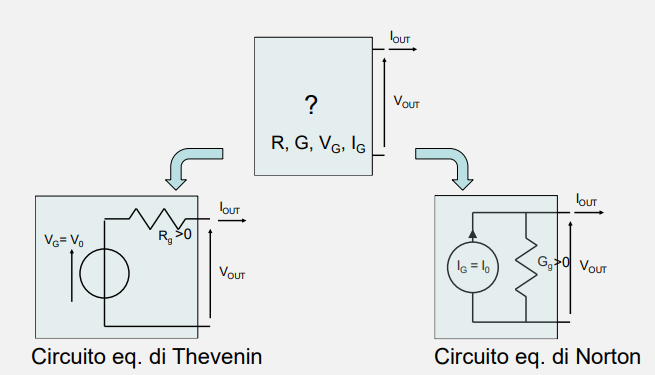
\includegraphics[scale=0.6]{IM_Thevenin_Norton_ter}
  \caption{Ogni rete elettrica ha 2 equivalenti circuitali}
  \label{Schema_Thevenin_Norton_ter}
\end{figure}

\begin{figure}[h]
  \centering
  %\captionsetup{justification=centering,margin=2cm}
  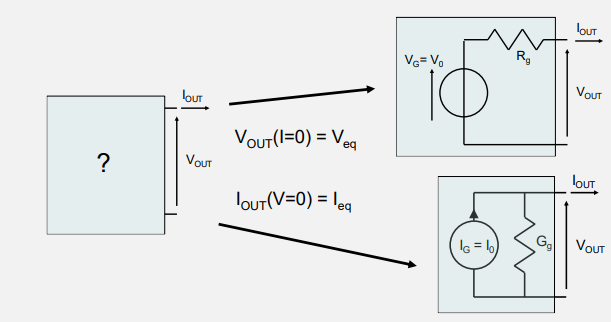
\includegraphics[scale=0.65]{IM_Thevenin_Norton_quater}
  \caption{Modelli equivalenti di una generica rete LTI (Linear Time-Invariant)}
  \label{Schema_Thevenin_Norton_quater}
\end{figure}

\textbf{Nota importante:} nella realtà del laboratorio i circuiti non sopportano tutto. Bisogna fare attenzione a come vengono fatti i collegamenti per evitare macelli.

\vspace{1mm}

Se ci si aspetta che un circuito ignoto sia un generatore di tensione, sarà ragionevolmente sicuro misurare $V_{eq}$ (ma non $I_{eq}$). Viceversa, se ci si aspetta che sia un generatore di corrente, sarà ragionevolmente sicuro misurare $I_{eq}$ (ma non $V_{eq}$). Leggere sempre e comunque le istruzioni d'uso dei componenti prima di fare qualunque cosa.

\vspace{1mm}

Nella realtà, per determinare l'equivalenza di due circuiti, ci si muove all'inerno di un ristretto intervallo di parametri:

\begin{itemize}
  \item per i generatori di tensione: $|I_{eq}|<I_{max}$
  \item per i generatori di corrente: $|V_{eq}|<V_{max}$
\end{itemize}

\textit{Esempio}: il caricatore del cellulare (USB) è equivalente ad un generatore di tensione (reale), con differenza di potenziale in uscita pari a $V_{OUT} = +5\,$V e corrente in uscita $I_{OUT} < 1\,$A.

\clearpage








\subsection{Impedenza di sorgente, di carico ed effetto di carico}

\begin{figure}[h]
  \centering
  %\captionsetup{justification=centering,margin=2cm}
  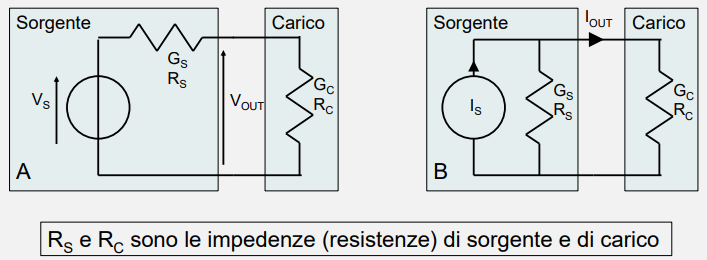
\includegraphics[scale=0.6]{IM_impedenze}
  \caption{Impedenze di sorgente e di carico}
  \label{Schema_impedenze}
\end{figure}

Ad un generatore di tensione è possibile collegare carichi diversi. Il carico ``migliore'' che è possibile collegare al generatore di tensione è il carico cosiddetto ``ideale'' (non collegare, cioè avere una resistenza infinita), mentre il carico ``peggiore'', in questo senso, è il cortocircuito (collegare una resistenza nulla). Quest'ultimo carico è particolarmente problematico perché, facendo fluire liberamente la corrente ai due capi del generatore, ``impedisce'' al generatore di imporre una differenza di potenziale ai suoi due capi. Un generatore vero potrebbe rompersi.

\vspace{3mm}

Nel caso invece del generatore di corrente, il carico ideale è il cortocircuito, poiché permette alla corrente da questo generata di fluire liberamente, mentre il carico peggiore è una resistenza infinita (non collegare), perché la corrente generata non può andare da nessuna parte. 

\vspace{3mm}

Con l'espressione \textit{togliere il carico} si intende, per il generatore di tensione, scollegare; per il generatore di corrente, cortocircuitare.

\begin{figure}[h]
  \centering
  %\captionsetup{justification=centering,margin=2cm}
  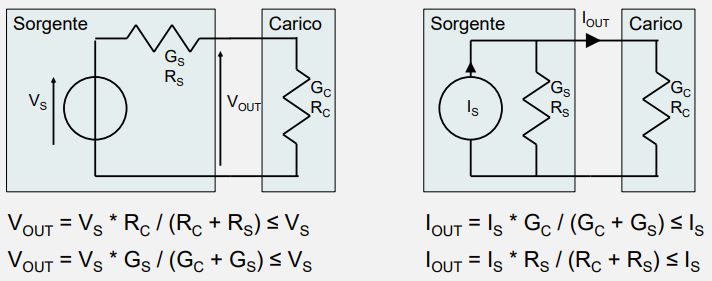
\includegraphics[scale=0.6]{IM_effetto_di_carico}
  \caption{Effetto di carico}
  \label{Schema_effetto_di_carico}
\end{figure}

Con l'espressione \textit{effetto di carico} si intende l'effetto per il quale, collegando un carico non ideale ad un generatore:

\begin{itemize}
\item di tensione, la tensione effettiva $V_{OUT}$ generata è minore, in modulo, rispetto al valore $V_S$ idealmente prodotto dal generatore
\item di corrente, la corrente effettiva $I_{OUT}$ generata è minore, in modulo, rispetto al valore $I_S$ idealmente prodotto dal generatore
\end{itemize}
\clearpage
L'effetto di carico non sarebbe presente se non esistesse la resistenza $R_S$, ovvero se ci trovassimo in presenza di un \textit{generatore ideale}. Purtroppo questi generatori non esistono.

\begin{figure}[h]
  \centering
  %\captionsetup{justification=centering,margin=2cm}
  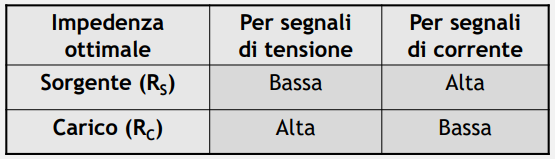
\includegraphics[scale=0.7]{IM_impedenza_ottimale}
  \caption{Tabella dell'impedenza ottimale}
  \label{Schema_impedenza_ottimale}
\end{figure}

È possible tuttavia provare a limitare questo effetto entro dei limiti accettabili, cercando di ridurre i termini moltiplicativi $R_C/(R_C + R_S)$ e $R_S/(R_C + R_S)$.

\vspace{1mm}

Per limitare l’effetto di carico è quindi opportuno avere:
\[R_C >> R_S \quad \textrm{per generatori di tensione}\]
\[R_C << R_S \quad \textrm{per generatori di corrente}\]










\subsection{Caratterizzazione degli elementi R, L, C nel dominio della frequenza}

\begin{figure}[h]
  \centering
  %\captionsetup{justification=centering,margin=2cm}
  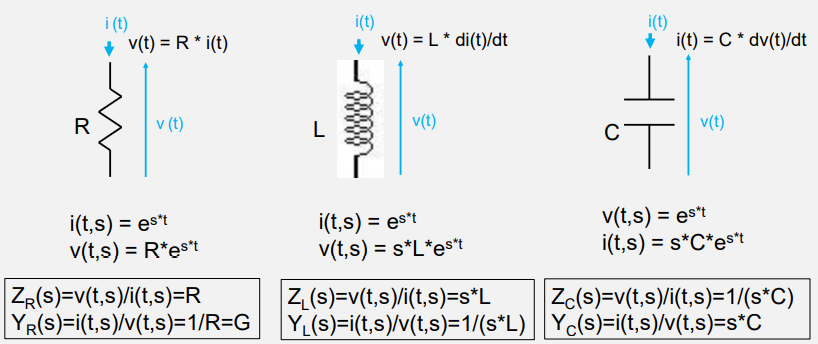
\includegraphics[scale=0.7]{IM_elementi_RLC_bis}
  \caption{Gli elementi RLC}
  \label{Schema_elementi_RLC}
\end{figure}

dove 
\begin{itemize}
  \item $s$ è una variabile complessa;
  \item abbiamo ipotizzato che la corrente segua l'evoluzione $i(t,s) = e^{s \cdot t}$ per la resistenza e per l'induttore;
  \item abbiamo ipotizzato che la tensione segua l'evoluzione $v(t,s) = e^{s \cdot t}$ per il condensatore.
\end{itemize}

Otteniamo così l'\textit{impedenza} $Z$, che si misura in ohm, e l'\textit{ammettenza} $Y$, che si misura in siemens. Queste due grandezza sono legate dalla relazione $Z=Y^{-1}$. Essendo tuttavia il parametro $s$ complesso, anche le grandezze $Z$ e $Y$ sono complesse.

\vspace{1mm}

D'ora in avanti, per evitare fraintendimenti con l'intensità di corrente, l'unità immaginaria verrà indicata con il simbolo $j$.

\vspace{1mm}

Ricordiamo la \textit{formula di Eulero}:

\[e^{st}= e^{(\sigma + j \cdot 2\pi f)t}= e^{\sigma t}(\textrm{cos} (2\pi f \cdot t) + j\textrm{sin} (2\pi f \cdot t))\]

Se $s = j\omega \Rightarrow e^{st} = \textrm{cos} (\omega t) + j\textrm{sin} (\omega t) \Rightarrow |e^{st}| = 1 \;\, \forall t \in \mathbb{R}$

\vspace{1mm}

Definiamo la fase di un numero complesso come
\[\measuredangle (a+jb) = \textrm{atan}\, (b/a)\]
Abbiamo quindi che:
\begin{itemize}
  \item $Z_R (j\omega) = R \Rightarrow |Z_R (j\omega)| = R$ e $\measuredangle (Z_R (j\omega)) = 0$
  \item $Z_L (j\omega) = j\omega L \Rightarrow |Z_L (j\omega)| = \omega L$ e $\measuredangle (Z_L (j\omega)) = \frac{\pi}{2}$
  \item $Z_C (j\omega) = 1/(j\omega C) \Rightarrow |Z_C (j\omega)| = 1/(\omega C)$ e $\measuredangle (Z_C (j\omega)) = -\frac{\pi}{2}$
\end{itemize}

In queste formule è possibile apprezzare la dualità tra condensatore e induttore.

\begin{figure}[h]
  \centering
  %\captionsetup{justification=centering,margin=2cm}
  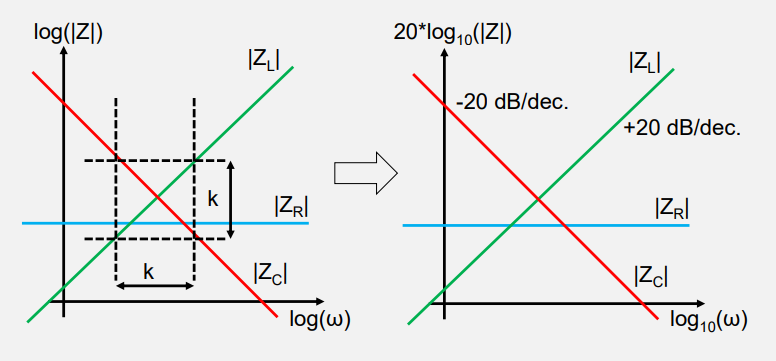
\includegraphics[scale=0.7]{IM_grafico_impedenze}
  \caption{Grafico impedenze}
  \label{Schema_grafico_impedenze}
\end{figure}

\clearpage












\subsection{I sistemi lineari, tempo invarianti}

Un sistema lineare è più complesso di un dipolo. Possiamo vederlo, per il momento, come un doppio dipolo.

\begin{figure}[h]
  \centering
  %\captionsetup{justification=centering,margin=2cm}
  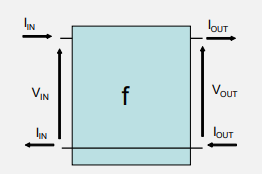
\includegraphics[scale=0.7]{IM_doppio_dipolo}
  \caption{Un doppio dipolo}
  \label{Schema_doppio_dipolo}
\end{figure}

Un doppio dipolo ha quattro gradi di libertà, due tensioni e due correnti. I segnali in ingresso e in uscita nel sistema possono essere sia tensioni che correnti. Il doppio dipolo schematizzato in figura \ref{Schema_doppio_dipolo} è un caso particolare, essendo i due poli raffigurati in basso equipotenziali (essendoci un collegamento diretto tra di loro). 

\vspace{3mm}

Ma cos'è un \textit{sistema lineare}? Dato un sistema $f$, dotato di un ingresso (formato eventualmente anche da un certo numero di entrate elementari) ed un'uscita, questo è lineare se e solo se l'uscita è combinazione lineare delle uscite che il sistema avrebbe applicandogli i singoli ingressi elementari:

\[f(C_1 \cdot IN_1 + C_2 \cdot IN_2) = C_1 \cdot f(IN_1) + C_2 \cdot f(IN_2)\]

$f$ è un sistema tempo invariante se e solo se le sue proprietà non dipendono dal tempo.

\vspace{3mm}

È detta \textit{funzione di trasferimento} (FdT) la relazione ($H$), espressa nei domini trasformati di Laplace ($s$) o di Fourier ($f$, $\omega$), tra un ingresso e un’uscita di $f$.

\begin{figure}[h]
  \centering
  %\captionsetup{justification=centering,margin=2cm}
  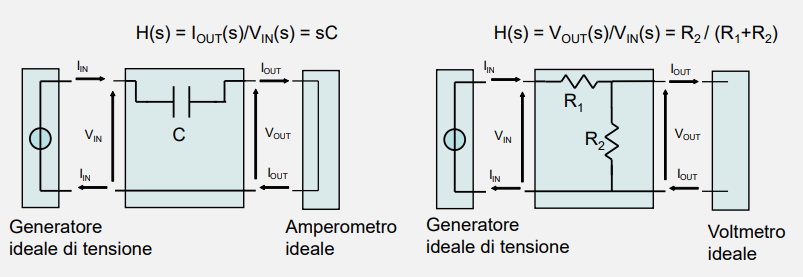
\includegraphics[scale=0.7]{IM_funzioni_trasferimento}
  \caption{Esempi di funzioni di trasferimento in doppi bipoli}
  \label{Schema_funzioni_trasferimento}
\end{figure}

Nel caso del primo circuito, la funzione di trasferimento $H(s)$ è la relazione tra un'entrata di tensione e un'uscita di corrente. La FdT è quindi l'ammettenza del condensatore.

\vspace{1mm}

Nel caso del secondo circuito è collegato al doppio dipolo un voltmetro ideale, a impedenza infinita, che misura la differenza di potenziale ai capi della resistenza $R_2$. La FdT $H(s)$ è il rapporto di partizione tra la resistenza $R_1$ e la resistenza $R_2$.

\begin{figure}[h]
  \centering
  %\captionsetup{justification=centering,margin=2cm}
  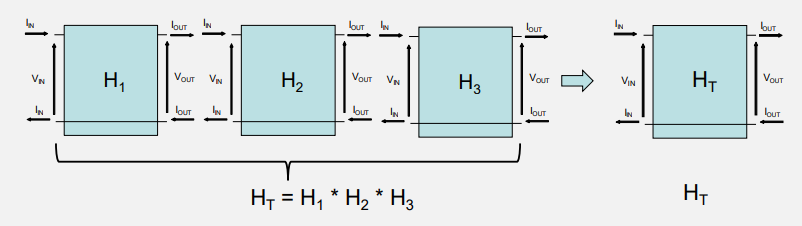
\includegraphics[scale=0.7]{IM_circuito_complesso}
  \caption{Un circuito complesso, modellizzato con 3 blocchi in cascata}
  \label{Schema_circuito_complesso}
\end{figure}

Il concetto di doppio dipolo e di FdT è importante per l'analisi di circuiti complessi. Un circuito è generalmente modellizzabile in blocchi, posti in cascata uno dopo l'altro. 

\vspace{1mm}

In assenza di effetti di carico (o se le singole Funzioni di Trasferimento sono ricavate considerando le impedenze di sorgente e di carico), la FdT complessiva corrisponde al prodotto delle singole FdT.

\vspace{1mm}

È possibile definire le proprietà di questi sistemi anche nel dominio del tempo.

\begin{figure}[h]
  \centering
  %\captionsetup{justification=centering,margin=2cm}
  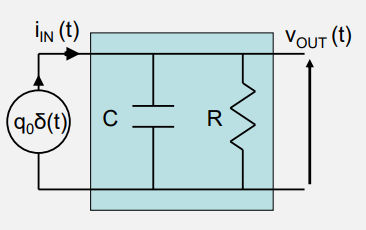
\includegraphics[scale=0.7]{IM_doppio_dipolo_tempo}
  \caption{Sistema caratterizzato nel tempo}
  \label{Schema_doppio_dipolo_tempo}
\end{figure}

Carichiamo il condensatore con un generatore di corrente che ha andamento impulsivo. La corrente emessa dal generatore è nulla per ogni $t$ diverso da 0 mentre, se $t=0$, il generatore emette un impulso di corrente che carica il condensatore di una carica $q_0$. 

\[i_{IN} = \delta (t) \cdot (C \cdot  v_0)\]

\[v_{OUT} = v_0 \cdot  e^{-t/(CR)}\]

Il sistema è lineare, quindi immettendo in ingresso una corrente generica $\delta (t)$

\[i_{IN} = \delta (t)\]

\[v_{OUT} = (1 / C) \cdot  e^{-t/(CR)} = h(t)\]

dove $h(t)$ è la risposta all'impulso $\delta(t)$ di un sistema lineare e tempo invariante.

\clearpage
Rappresentare la proprietà di un sistema LTI i termini di risposta all'impulso $h(t)$ o in termini di FdT $H(f)$ consente di rappresentare la risposta del sistema LTI (Linear Time-Invariant) per qualsiasi segnale in ingresso, posto che questo sia a sua volta rappresentabile sulla base di impulsi di Dirac o di funzioni armoniche:

\[in(t) = \int_{-\infty}^{\infty} in(\xi) \cdot \delta (t - \xi) \cdot \textrm{d} \xi = \int_{-\infty}^{\infty} IN (f) \cdot e^{j \omega f t} \cdot \textrm d f\]

\begin{figure}[h]
  \centering
  %\captionsetup{justification=centering,margin=2cm}
  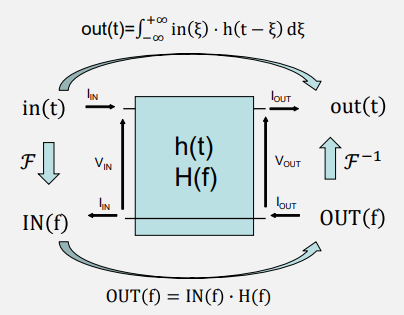
\includegraphics[scale=0.7]{IM_trasformata_fourier}
  \caption{Sistema caratterizzato nel tempo}
  \label{Schema_trasformata_fourier}
\end{figure}

Definiamo la \textit{trasformata di Fourier} ($\mathcal{F}$) e la sua \textit{anti-trasformata} ($\mathcal{F}^{-1}$)

\[IN (f) = \mathcal{F} (in(t)) = \int_{-\infty}^{\infty} in(t) \cdot e^{-j2\pi ft} \cdot \textrm d t\]

\[in (t) = \mathcal{F}^{-1} (IN(f)) = \int_{-\infty}^{\infty} IN(t) \cdot e^{j2\pi ft} \cdot \textrm d t\]

Consegue infine che:

\[h(t) \underset{\mathcal{F}^{-1}}{\overset{\mathcal{F}}{\rightleftarrows}} H(f)\]

\clearpage












\section{Circuiti passivi con elementi RLC}

Da questo capitolo apparirà il simbolo formato da tre linee di lunghezza decrescente (figura \ref{GND}). Questo rappresenta la messa a massa o GND. Questo funge da generico punto di riferimento per la misura delle differenze di potenziale. È utile quando si lavora con il simulatore circuitale per potere indicare con facilità l'equipotenzialità di parti del circuito graficamente molto distanti. 

\begin{figure}[h]
  \centering
  %\captionsetup{justification=centering,margin=2cm}
  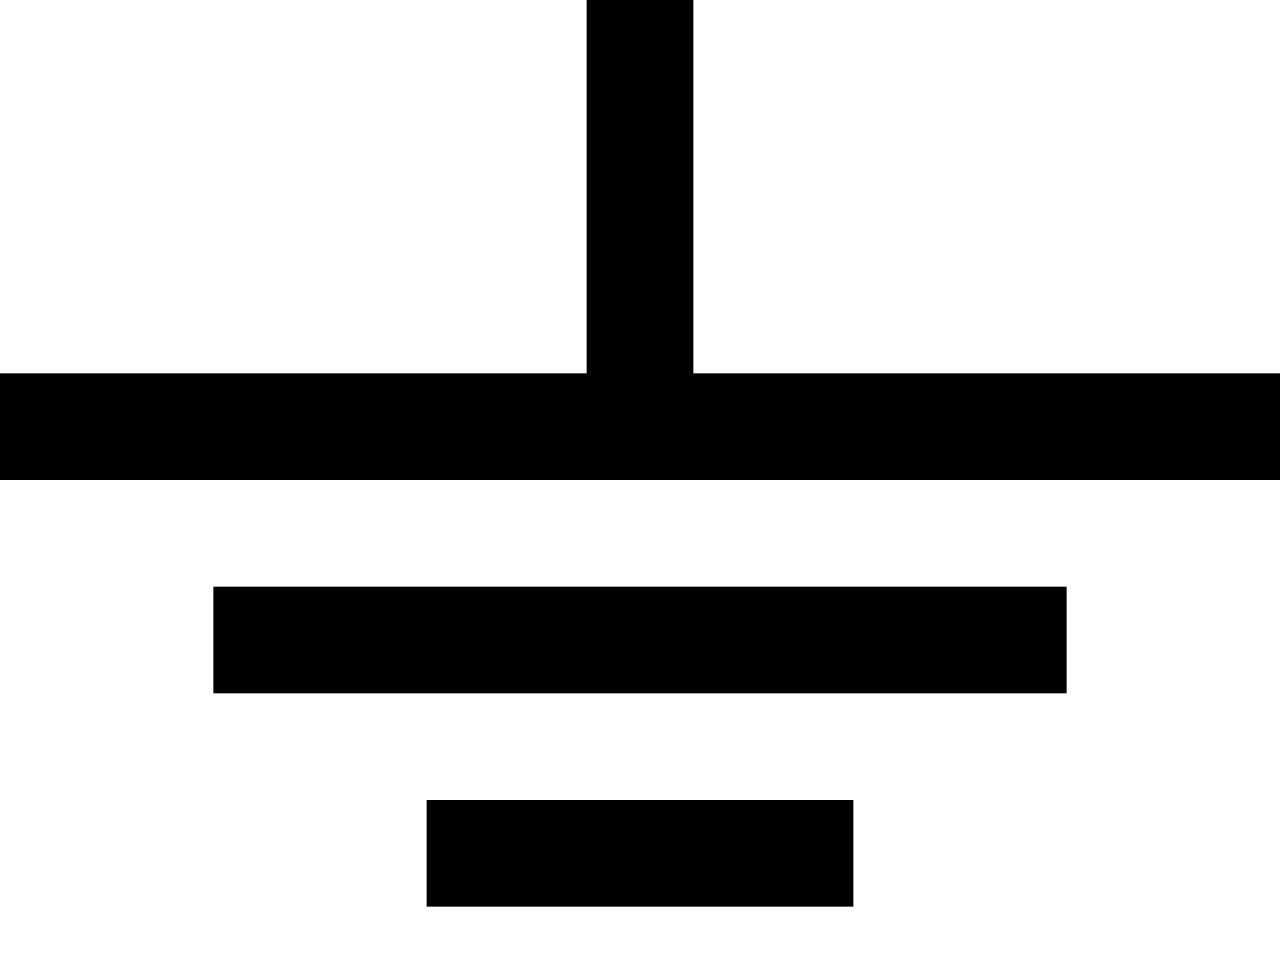
\includegraphics[scale=0.1]{IM_GND.png}
  \caption{Rappresentazione grafica del GND}
  \label{GND}
\end{figure}

\subsection{Circuiti RC e RL}

L'analisi nel dominio della frequenza sarà la più semplice e diretta, applicando i concetti di partitore di tensione e di corrente alle impedenze.

\begin{figure}[h]
  \centering
  %\captionsetup{justification=centering,margin=2cm}
  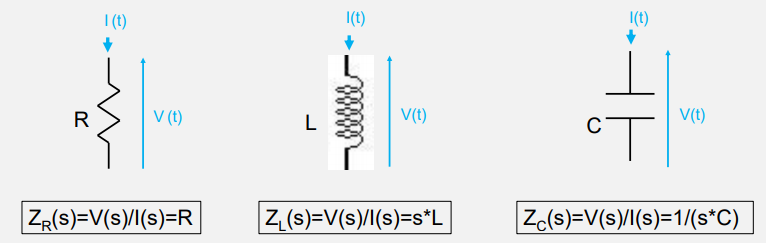
\includegraphics[scale=0.7]{IM_impedenze_bis}
  \caption{Le impedenze}
  \label{Schema_impedenze_bis}
\end{figure}
\clearpage
Cominciamo con il circuito RC (\textit{Filtro passa basso RC passivo}) in figura \ref{Schema_circuito_RC_passivo}.
\begin{figure}[h]
  \centering
  %\captionsetup{justification=centering,margin=2cm}
  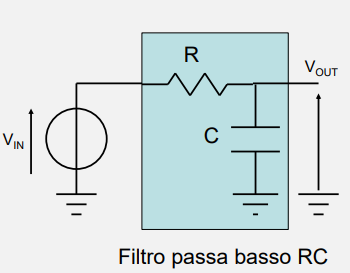
\includegraphics[scale=0.6]{IM_circuito_RC_passivo}
  \caption{Circuito RC}
  \label{Schema_circuito_RC_passivo}
\end{figure}

Generalizzando alle impedenze quanto visto per le resistenze:
\[V_{OUT}(s) = V_{IN}(s) \cdot \frac{Z_C(s)}{Z_C(s) + Z_R(s)}\]
da cui 
\[H(s) = \frac{V_{OUT} (s)}{V_{IN} (s)} = \frac{Z_C(s)}{Z_C(s) + Z_R(s)}\]
sostituendo adesso alle impedenze le loro espressioni esplicite:
\[H(s) = \frac{1/sC}{1/sC + R} = \frac{1}{1 + sRC}\]
e, per $s = j\omega$, 
\[H(s) = \frac{1}{1 + j \omega RC} \quad \quad |H(s)| = \frac{1}{\sqrt{1 + \omega ^2 \cdot R^2 \cdot C^2}} \quad \quad \measuredangle (H(j \omega)) = \textrm{atan}\, (- \omega RC)\]
\begin{figure}[h]
  \centering
  %\captionsetup{justification=centering,margin=2cm}
  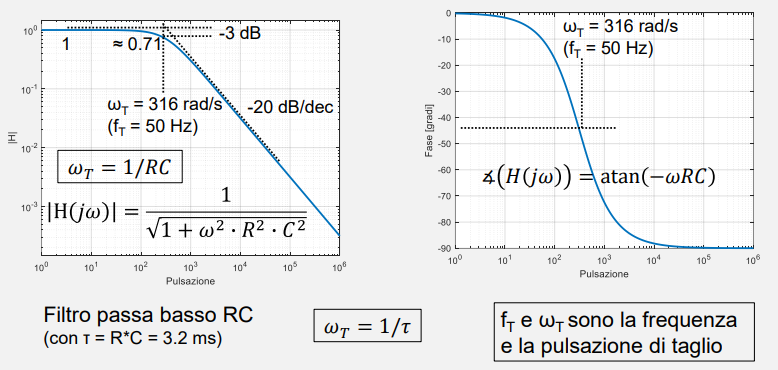
\includegraphics[scale=0.6]{IM_circuito_RC_passivo_grafici}
  \caption{La funzione di trasferimento al variare della pulsazione}
  \label{Schema_circuito_RC_passivo_grafici}
\end{figure}
\clearpage
Concentrandoci ora sul circuito CR (\textit{Filtro passa alto CR attivo}) in figura \ref{Schema_circuito_CR_passivo}:

\begin{figure}[h]
  \centering
  %\captionsetup{justification=centering,margin=2cm}
  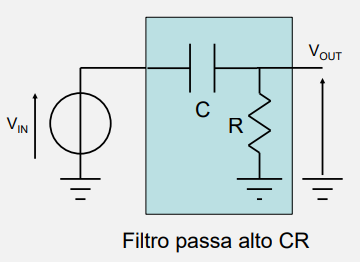
\includegraphics[scale=0.6]{IM_circuito_CR_passivo}
  \caption{Circuito CR}
  \label{Schema_circuito_CR_passivo}
\end{figure}
si ha
\[V_{OUT}(s) = V_{IN}(s) \cdot \frac{Z_C(s)}{Z_C(s) + Z_R(s)}\]
da cui 
\[H(s) = \frac{V_{OUT} (s)}{V_{IN} (s)} = \frac{Z_C(s)}{Z_C(s) + Z_R(s)}\]
sostituendo adesso alle impedenze le loro espressioni esplicite:
\[H(s) = \frac{R}{R + 1/sC} = \frac{sRC}{1 + sRC}\]
e, per $s = j\omega$, 
\[H(s) = \frac{j \omega RC}{1 + j \omega RC} \quad \quad |H(s)| = \frac{\omega RC}{\sqrt{1 + \omega ^2 \cdot R^2 \cdot C^2}} \quad \quad \measuredangle (H(j \omega)) = \textrm{atan}\, \left(\frac{1}{\omega RC}\right)\]

\begin{figure}[h]
  \centering
  %\captionsetup{justification=centering,margin=2cm}
  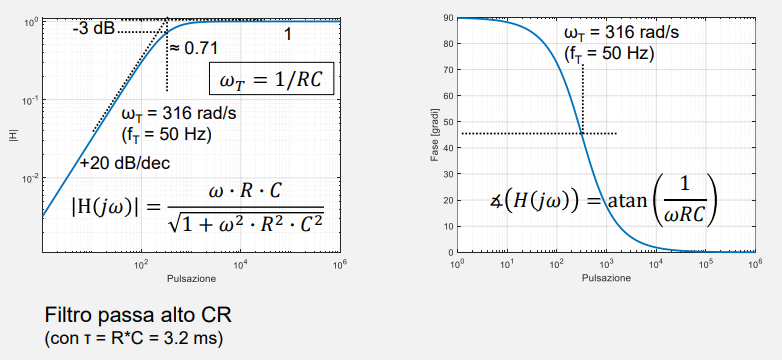
\includegraphics[scale=0.7]{IM_circuito_CR_passivo_grafici}
  \caption{La funzione di trasferimento al variare della pulsazione}
  \label{Schema_circuito_CR_passivo_grafici}
\end{figure}
\clearpage
Analogamente si procede per le induttanze. Con il circuito RL in figura \ref{Schema_circuito_RL_passivo} (\textit{Filtro passa alto RL passivo}):

\begin{figure}[h]
  \centering
  %\captionsetup{justification=centering,margin=2cm}
  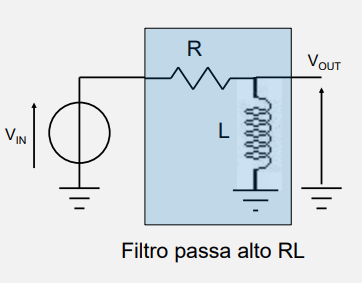
\includegraphics[scale=0.6]{IM_circuito_RL_passivo}
  \caption{Circuito RL}
  \label{Schema_circuito_RL_passivo}
\end{figure}

si ha
\[V_{OUT}(s) = V_{IN}(s) \cdot \frac{Z_L(s)}{Z_L(s) + Z_R(s)}\]
da cui 
\[H(s) = \frac{V_{OUT} (s)}{V_{IN} (s)} = \frac{Z_L(s)}{Z_L(s) + Z_R(s)}\]
sostituendo adesso alle impedenze le loro espressioni esplicite:
\[H(s) = \frac{sL}{sL + R} = \frac{sL/R}{1 + sL/R}\]
e, per $s = j\omega$, 
\[H(s) = \frac{j \omega L/R}{1 + j \omega L/R} \quad \quad |H(s)| = \frac{\omega L/R}{\sqrt{1 + \omega ^2 \cdot L^2 / R^2}} \quad \quad \measuredangle (H(j \omega)) = \textrm{atan}\, \left(\frac{R}{\omega L} \right)\]

\begin{figure}[h]
  \centering
  %\captionsetup{justification=centering,margin=2cm}
  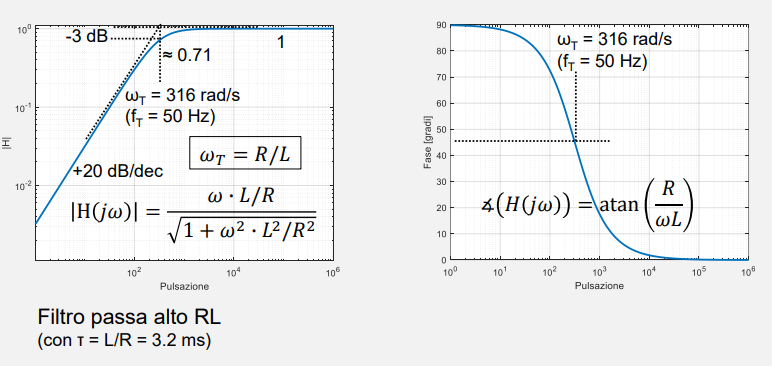
\includegraphics[scale=0.6]{IM_circuito_RL_passivo_grafici}
  \caption{La funzione di trasferimento al variare della pulsazione}
  \label{Schema_circuito_RL_passivo_grafici}
\end{figure}
\clearpage
Concentrandoci ora sul circuito LR in figura \ref{Schema_circuito_LR_passivo} (\textit{Filtro passa basso RL passivo}):

\begin{figure}[h]
  \centering
  %\captionsetup{justification=centering,margin=2cm}
  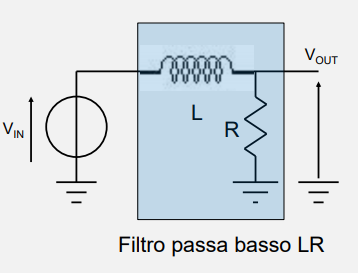
\includegraphics[scale=0.55]{IM_circuito_LR_passivo}
  \caption{Circuito LR}
  \label{Schema_circuito_LR_passivo}
\end{figure}

si ha
\[V_{OUT}(s) = V_{IN}(s) \cdot \frac{Z_R(s)}{Z_L(s) + Z_R(s)}\]
da cui 
\[H(s) = \frac{V_{OUT} (s)}{V_{IN} (s)} = \frac{Z_R(s)}{Z_L(s) + Z_R(s)}\]

sostituendo adesso alle impedenze le loro espressioni esplicite:
\[H(s) = \frac{R}{R + sL} = \frac{1}{1 + sL/R}\]
e, per $s = j\omega$, 
\[H(s) = \frac{1}{1 + j \omega L/R} \quad \quad |H(s)| = \frac{1}{\sqrt{1 + \omega ^2 \cdot L^2 / R^2}} \quad \quad \measuredangle (H(j \omega)) = \textrm{atan}\, \left(-\frac{\omega L}{ R}\right)\]

\begin{figure}[h]
  \centering
  %\captionsetup{justification=centering,margin=2cm}
  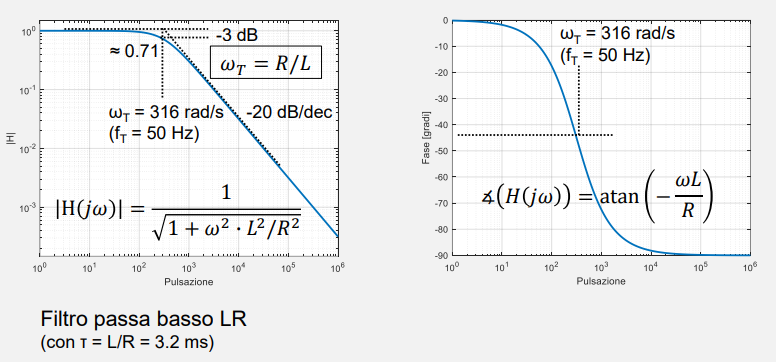
\includegraphics[scale=0.7]{IM_circuito_LR_passivo_grafici}
  \caption{La funzione di trasferimento al variare della pulsazione}
  \label{Schema_circuito_LR_passivo_grafici}
\end{figure}

\clearpage










\subsection{Circuiti risonanti serie}

Concentrandoci ora sul circuito LC mostrato in figura \ref{Schema_circuito_risonante_serie_LC} (\textit{Filtro risonante serie LC passivo}).

\begin{figure}[h]
  \centering
  %\captionsetup{justification=centering,margin=2cm}
  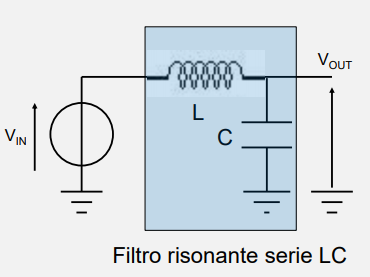
\includegraphics[scale=0.5]{IM_circuito_risonante_serie_LC}
  \caption{Circuito risonante serie LC}
  \label{Schema_circuito_risonante_serie_LC}
\end{figure}

\[V_{OUT}(s) = V_{IN}(s) \cdot \frac{Z_C(s)}{Z_L(s) + Z_C(s)}\]

da cui

\[H(s) = \frac{V_{OUT} (s)}{V_{IN} (s)} = \frac{Z_C(s)}{Z_L(s) + Z_C(s)}\]

sostituendo adesso alle impedenze le loro espressioni esplicite:

\[H(s) = \frac{1/sC}{1/sC + sL} = \frac{1}{1 + s^2 LC}\]

e, per $s = j\omega$, 

\[H(s) = \frac{1}{1 - \omega ^2 LC} \quad \quad |H(s)| = \begin{cases} \frac{1}{1 - \omega ^2 \cdot LC} \textrm{ se } \omega < \frac{1}{\sqrt{LC}} \\ \frac{1}{\omega ^2 \cdot LC - 1} \textrm{ se } \omega > \frac{1}{\sqrt{LC}} \end{cases} \quad \quad \measuredangle (H(j \omega)) = \begin{cases} 0 \textrm{ se } \omega < \frac{1}{\sqrt{LC}} \\ \pm \pi \textrm{ se } \omega > \frac{1}{\sqrt{LC}} \end{cases}\]

\begin{figure}[h]
  \centering
  %\captionsetup{justification=centering,margin=2cm}
  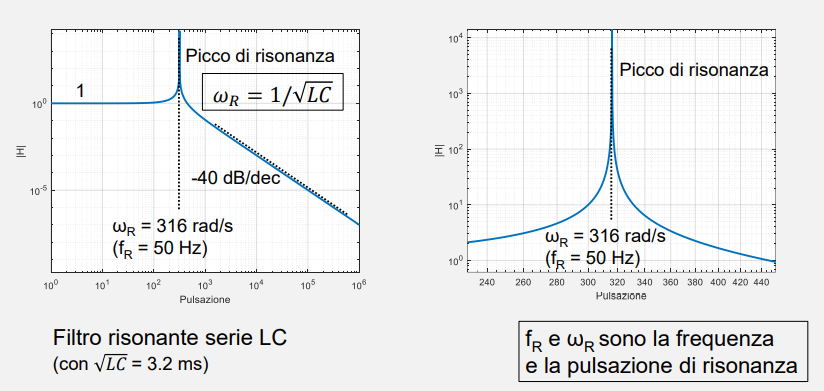
\includegraphics[scale=0.55]{IM_circuito_risonante_serie_LC_grafici}
  \caption{La funzione di trasferimento al variare della pulsazione}
  \label{Schema_circuito_risonante_serie_LC_grafici}
\end{figure}

\clearpage
Concentrandoci ora sul circuito CL mostrato in figura \ref{Schema_circuito_risonante_serie_CL} (\textit{Filtro risonante serie CL passivo}):

\begin{figure}[h]
  \centering
  %\captionsetup{justification=centering,margin=2cm}
  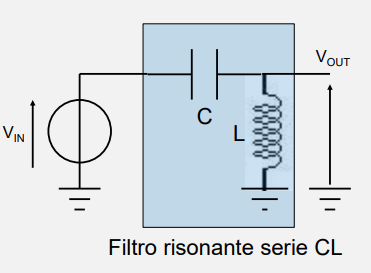
\includegraphics[scale=0.5]{IM_circuito_risonante_serie_CL}
  \caption{Circuito risonante serie CL}
  \label{Schema_circuito_risonante_serie_CL}
\end{figure}

\[V_{OUT}(s) = V_{IN}(s) \cdot \frac{Z_L(s)}{Z_L(s) + Z_C(s)}\]

da cui

\[H(s) = \frac{V_{OUT} (s)}{V_{IN} (s)} = \frac{Z_L(s)}{Z_L(s) + Z_C(s)}\]

sostituendo adesso alle impedenze le loro espressioni esplicite:

\[H(s) = \frac{sL}{1/sC + sL} = \frac{s^2 LC}{1 + s^2 LC}\]

e, per $s = j\omega$, 

\[H(s) = -\frac{\omega ^2 LC}{1 - \omega ^2 LC} \quad \quad |H(s)| = \begin{cases} \frac{\omega ^2 \cdot LC}{1 - \omega ^2 \cdot LC} \textrm{ se } \omega < \frac{1}{\sqrt{LC}} \\ \frac{\omega ^2 \cdot LC}{\omega ^2 \cdot LC - 1} \textrm{ se } \omega > \frac{1}{\sqrt{LC}} \end{cases} \quad \quad \measuredangle (H(j \omega)) = \begin{cases} \pm \pi \textrm{ se } \omega < \frac{1}{\sqrt{LC}} \\ 0 \textrm{ se } \omega > \frac{1}{\sqrt{LC}} \end{cases}\]

\begin{figure}[h]
  \centering
  %\captionsetup{justification=centering,margin=2cm}
  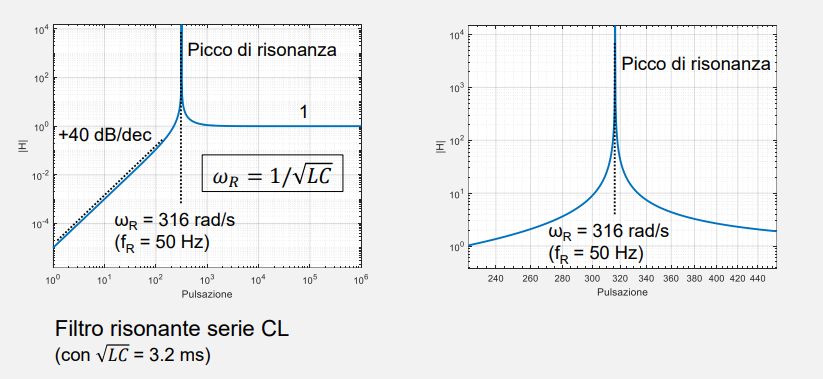
\includegraphics[scale=0.55]{IM_circuito_risonante_serie_CL_grafici}
  \caption{La funzione di trasferimento al variare della pulsazione}
  \label{Schema_circuito_risonante_serie_CL_grafici}
\end{figure}

\clearpage
Concentrandoci ora sul circuito RLC mostrato in figura \ref{Schema_circuito_risonante_serie_RLC} (\textit{Filtro risonante serie RLC passivo}):

\begin{figure}[h]
  \centering
  %\captionsetup{justification=centering,margin=2cm}
  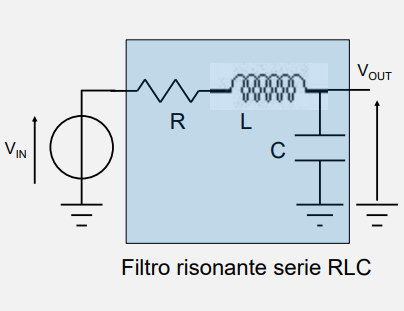
\includegraphics[scale=0.48]{IM_circuito_risonante_serie_RLC}
  \caption{Circuito risonante serie RLC}
  \label{Schema_circuito_risonante_serie_RLC}
\end{figure}
\[V_{OUT}(s) = V_{IN}(s) \cdot \frac{Z_C(s)}{Z_R(s) + Z_L(s) + Z_C(s)}\]
da cui
\[H(s) = \frac{V_{OUT} (s)}{V_{IN} (s)} = \frac{Z_C(s)}{Z_R(s) + Z_L(s) + Z_C(s)}\]

sostituendo adesso alle impedenze le loro espressioni esplicite:

\[H(s) = \frac{1/sC}{1/sC + sL + R} = \frac{1}{1 + sRC + s^2 LC}\]

e, per $s = j\omega$, 

\[H(s) = \frac{1}{1 + j \omega RC - \omega ^2 LC} \quad \quad |H(s)| = \left| \frac{1}{\sqrt{(1 - \omega ^2 LC)^2 + (\omega RC)^2}} \right| \]

\[|H(s)|_{\omega = \omega_R} = \frac{1}{R} \cdot \sqrt{\frac{L}{C}} \approx P_R \quad \quad \textrm{dove } \omega _R = \frac{1}{\sqrt{LC}}\]

Per $R \geq 2 \cdot \sqrt{\frac{L}{C}}$ non ci sono effetti di risonanza.

\begin{figure}[h]
  \centering
  %\captionsetup{justification=centering,margin=2cm}
  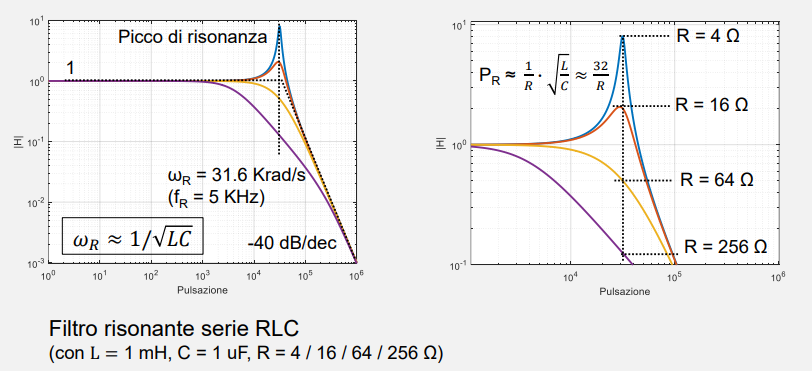
\includegraphics[scale=0.48]{IM_circuito_risonante_serie_RLC_grafici}
  \caption{La funzione di trasferimento al variare della pulsazione}
  \label{Schema_circuito_risonante_serie_RLC_grafici}
\end{figure}

Il fattore di merito (o qualità) $Q$ esprime la relativa prevalenza degli effetti risonanti / dissipativi:

\[Q = \frac{\omega _R}{\Delta \omega _{-3dB}} = \frac{1}{R} \cdot \sqrt{\frac{L}{C}}\]











\clearpage
\subsection{Circuiti risonanti parallelo}

Concentrandoci ora sul circuito LC mostrato in figura \ref{Schema_circuito_risonante_parallelo_LC} (\textit{Filtro risonante parallelo LC passivo}):

\begin{figure}[h]
  \centering
  %\captionsetup{justification=centering,margin=2cm}
  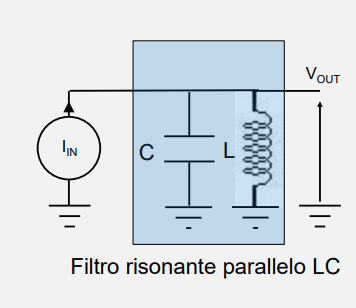
\includegraphics[scale=0.5]{IM_circuito_risonante_parallelo_LC}
  \caption{Circuito risonante parallelo LC}
  \label{Schema_circuito_risonante_parallelo_LC}
\end{figure}

\[V_{OUT}(s) = I_{IN}(s) \cdot (Z_C(s) // Z_L (s))\]

da cui

\[H(s) = \frac{V_{OUT} (s)}{I_{IN} (s)} = (Z_C(s) // Z_L (s))\]

sostituendo adesso alle impedenze le loro espressioni esplicite:

\[H(s) = \frac{1}{sC + 1/sL} = \frac{sL}{1 + s^2 LC}\]

e, per $s = j\omega$, 

\[H(s) = \frac{j \omega L}{1 - \omega ^2 LC} \quad \quad |H(s)| = \begin{cases} \frac{\omega \cdot L}{1 - \omega ^2 \cdot LC} \textrm{ se } \omega < \frac{1}{\sqrt{LC}} \\ \frac{\omega \cdot L}{\omega ^2 \cdot LC - 1} \textrm{ se } \omega > \frac{1}{\sqrt{LC}} \end{cases} \quad \quad \measuredangle (H(j \omega)) = \begin{cases} + \frac{\pi}{2} \textrm{ se } \omega < \frac{1}{\sqrt{LC}} \\ - \frac{\pi}{2} \textrm{ se } \omega > \frac{1}{\sqrt{LC}} \end{cases}\]

\begin{figure}[h]
  \centering
  %\captionsetup{justification=centering,margin=2cm}
  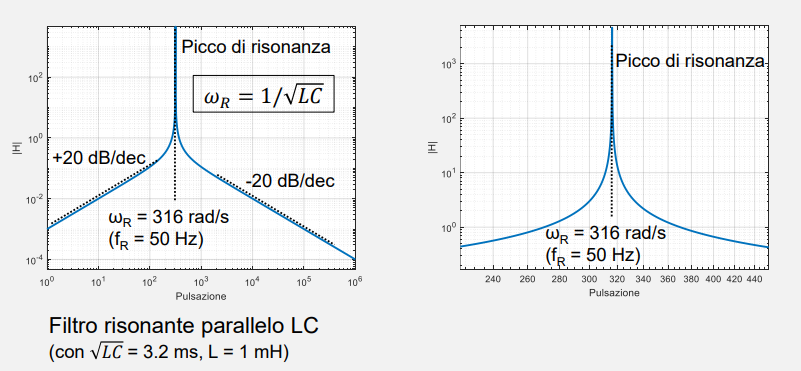
\includegraphics[scale=0.55]{IM_circuito_risonante_parallelo_LC_grafici}
  \caption{La funzione di trasferimento al variare della pulsazione}
  \label{Schema_circuito_risonante_parallelo_LC_grafici}
\end{figure}
\clearpage
Concentrandoci ora sul circuito RLC mostrato in figura \ref{Schema_circuito_risonante_parallelo_RLC} (\textit{Filtro risonante parallelo RLC passivo}):

\begin{figure}[h]
  \centering
  %\captionsetup{justification=centering,margin=2cm}
  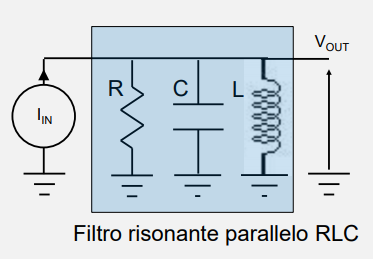
\includegraphics[scale=0.5]{IM_circuito_risonante_parallelo_RLC}
  \caption{Circuito risonante parallelo RLC}
  \label{Schema_circuito_risonante_parallelo_RLC}
\end{figure}

\[V_{OUT}(s) = I_{IN}(s) \cdot (Z_C(s) // Z_L (s) // Z_R (s))\]

da cui

\[H(s) = \frac{V_{OUT} (s)}{I_{IN} (s)} = (Z_C(s) // Z_L (s) // Z_R (s))\]

sostituendo adesso alle impedenze le loro espressioni esplicite:

\[H(s) = \frac{1}{sC + 1/sL + 1/R} = \frac{sL}{1 + sL/R + s^2 LC}\]

e, per $s = j\omega$, 

\[H(s) = \frac{j \omega L}{1 + j \omega L/R - \omega ^2 LC} \quad \quad |H(s)| = \left| \frac{\omega L}{\sqrt{(1 - \omega ^2 LC)^2 + (\omega L/R)^2}} \right| \]

\[|H(s)|_{\omega = \omega_R} = R \approx P_R \quad \quad \textrm{dove } \omega _R = \frac{1}{\sqrt{LC}}\]

Per $R \geq \frac{1}{2} \cdot \sqrt{\frac{L}{C}}$ non ci sono effetti di risonanza.

\begin{figure}[h]
  \centering
  %\captionsetup{justification=centering,margin=2cm}
  \includegraphics[scale=0.5]{IM_circuito_risonante_parallelo_RLC_grafici}
  \caption{La funzione di trasferimento al variare della pulsazione}
  \label{Schema_circuito_risonante_parallelo_RLC_grafici}
\end{figure}

Il fattore di merito (o qualità) $Q$ esprime la relativa prevalenza degli effetti risonanti / dissipativi, e in questo caso vale:

\[Q = \frac{\omega _R}{\Delta \omega _{-3dB}} = R \cdot \sqrt{\frac{C}{L}}\]


\clearpage










\section{Circuiti attivi lineari con amplificatori operazionali}

\subsection{L’amplificatore operazionale}

\begin{figure}[h]
  \centering
  %\captionsetup{justification=centering,margin=2cm}
  \includegraphics[scale=0.7]{IM_amplificatore_operazionale}
  \caption{L'amplificatore operazionale}
  \label{Schema_amplificatore_operazionale}
\end{figure}

Un \textit{amplificatore operazionale} è un dispositivo ad almeno 5 terminali (anche se molto spesso ne ha un numero maggiore). Questi 5 terminali sono così suddivisi:
\begin{itemize}
  \item Due ingressi, tipicamente di tensione (esistono anche degli amplificatori operazionali detti ``current mode'' che hanno un ingresso di tensione e un ingresso di corrente);
  \item un'uscita di tensione;
  \item  due terminali di alimentazione.
\end{itemize}

\vspace{3mm}

È un dispositivo attivo. Un \textit{dispositivo attivo} è un dispositivo che trasferisce potenza dai terminali di alimentazione all'uscita. Una popolare definizione sbagliata di dispositivo attivo è quella di un dispositivo in cui l'uscita, in tensione, è maggiore degli ingressi applicati. Per accertarne la falsità è sufficiente pensare ad un circuito risonante che ha in ingresso un segnale alla frequenza di risonanza.

\vspace{3mm}

Un amplificatore operazionale ha due terminali di alimentazione: un terminale di alimentazione positiva e uno di alimentazione negativa (dove per positività e negatività non si intende che uno dà e l'altro assorbe, ma che uno dei due ``alimenta'' più dell'altro). È importante evitare di confondere i due terminali per evitare di danneggiare circuiti reali.

\begin{figure}[h]
  \centering
  %\captionsetup{justification=centering,margin=2cm}
  \includegraphics[scale=0.7]{IM_amplificatore_operazionale_ideale}
  \caption{L'amplificatore operazionale ideale}
  \label{Schema_amplificatore_operazionale_ideale}
\end{figure}

Un amplificatore operazionale ideale, ovvero la più semplice modellizzazione possibile di un amplificatore, ha:

\begin{itemize}
  \item Ingressi di tensione a impedenza infinita (non c'è passaggio di corrente)
  \item Uscita di tensione a impedenza nulla (generatore di tensione ideale)
  \item Alimentazione con differenza di potenziale infinita
  \item Modellizzabile con un sistema lineare:
  \[V_{OUT} = f(V_{IN+} - V_{IN-}) = f(\Delta V_{IN}) = A_0 \cdot \Delta V_{IN} \quad (A_0 \textrm{ cost.} \rightarrow \infty)\]
  \item Per valori finiti di $V_{OUT}$:
  \[\Delta V_{IN} = V_{OUT}/A_0 \rightarrow 0V \Rightarrow V_{IN+} \approx V_{IN-}\]
\end{itemize}

Un modello è valido quando riesce ad prevedere correttamente il comportamento di un sistema senza aggiungere complicazioni non necessarie. Il modello sovradescritto è sempre valido?

\begin{figure}[h]
  \centering
  %\captionsetup{justification=centering,margin=2cm}
  \includegraphics[scale=0.55]{IM_amplificatore_operazionale_modello}
  \caption{L'invalidità del modello}
  \label{Schema_amplificatore_operazionale_modello}
\end{figure}

No. Cambiando il potenziale di riferimento $V_R$ non cambio la differenza di potenziale tra i due ingressi, quindi il potenziale in uscita resta invariato. Ma questo, come visibile dai conti in figura \ref{Schema_amplificatore_operazionale_modello}, è un paradosso.

\begin{figure}[h]
  \centering
  %\captionsetup{justification=centering,margin=2cm}
  \includegraphics[scale=0.55]{IM_amplificatore_operazionale_modello_bis}
  \caption{Un modello alternativo}
  \label{Schema_amplificatore_operazionale_modello_bis}
\end{figure}

Il modello alternativo schematizzato in figura \ref{Schema_amplificatore_operazionale_modello_bis}, invece, resta valido al variare del potenziale di riferimento, ma non è realistico in quanto prevede un ulteriore terminale che l'amplificatore operazionale non ha.

\begin{figure}[h]
  \centering
  %\captionsetup{justification=centering,margin=2cm}
  \includegraphics[scale=0.6]{IM_amplificatore_operazionale_meno_ideale}
  \caption{Un amplificatore operazionale meno ideale}
  \label{Schema_amplificatore_operazionale_meno_ideale}
\end{figure}

Allontanandoci dal caso ideale e avvicinandosi a quello reale:

\begin{itemize}
  \item Guadagno finito: $A_0 >> 1$ (es. $10^4$ - $10^6$)
  \item Correnti all'ingresso non nulle ma trascurabili (di diversi ordini di grandezza più piccole rispetto alle altre correnti in gioco)
  \item Alimentazione con differenza di potenziale finita:
  \[\Delta V_{MIN} \leq V_{CC} + V_{EE} \leq \Delta V_{MAX} \quad \textrm{con} \; \Delta V_{MIN} > 0\]
  \item Potenziale in uscita limitato dalle alimentazioni:
  \[-V_{EE} + \Delta V_{EE} \leq V_{OUT} \leq + V_{CC} - \Delta V_{CC}\]
  con $\Delta V_{CC}$ e $\Delta V_{EE}$ compresi tra 0 e qualche Volt a seconda del tipo di Op. Amp. (Operational Amplifier)
  \item $V_{IN+} \approx V_{IN-}$, ma solo in certe condizioni
\end{itemize}

\begin{figure}[h]
  \centering
  %\captionsetup{justification=centering,margin=2cm}
  \includegraphics[scale=0.55]{IM_amplificatore_operazionale_grafico}
  \caption{Grafico della tensione in uscita in funzione della differenza di potenziale tra gli ingressi}
  \label{Schema_amplificatore_operazionale_grafico}
\end{figure}

Quando accade che $V_{IN+} \approx V_{IN-}$? Guardando il grafico in figura \ref{Schema_amplificatore_operazionale_grafico}, si evince che $\Delta x = \Delta y / A_0$: essendo $A_0$ molto grande ($10^4$ - $10^6$), la differenza di potenziale $\Delta x$ sarà piccola relativamente a $\Delta y$ e $V_{IN+} \approx V_{IN-}$ sarà verificata. Questo è vero fintantoché l'uscita non è in saturazione, ovvero dipende dagli ingressi. 

\vspace{2mm}

Quando l'uscita è in saturazione, essa è determinata dall'alimentazione e non dagli ingressi, e non varrà più la relazione sopra descritta; in questo caso è evidentemente possibile aumentare la differenza di potenziale $\Delta x$ fino all'ordine di grandezza di $\Delta y$ senza alcun effetto su quest'ultima.

\begin{figure}[h]
  \centering
  %\captionsetup{justification=centering,margin=2cm}
  \includegraphics[scale=0.45]{IM_amplificatore_operazionale_carta_e_penna}
  \caption{Modello di amplificatore operazionale ``carta e penna''}
  \label{Schema_amplificatore_operazionale_carta_e_penna}
\end{figure}
Un modello ``carta e penna'' di un amplificatore operazionale può essere come quello riportato in figura \ref{Schema_amplificatore_operazionale_carta_e_penna} e onestamente non troppo diverso dai primi schizzi visti in questa sezione.

Questo modello ha le seguenti caratteristiche: 
\begin{itemize}
  \item Potenziale in uscita limitato dalle alimentazioni:
  \[-V_{EE} \leq V_{OUT} \leq + V_{CC}\]
  (non sempre è possibile che l'uscita ``raggiunga'' le alimentazioni, ma per i fini di questo modello è un'assunzione ragionevole e la faremo)
  \item se l'uscita non è in saturazione, $V_{IN+} \approx V_{IN-}$
  \item Correnti agli ingressi trascurabili $I_{IN+} \approx I_{IN-} \approx 0$
\end{itemize}

\begin{figure}[h]
  \centering
  %\captionsetup{justification=centering,margin=2cm}
  \includegraphics[scale=0.57]{IM_amplificatore_operazionale_reale}
  \caption{Modello di Op. Amp. più realistico, che funziona sempre, ma è anche più complicato...}
  \label{Schema_amplificatore_operazionale_reale}
\end{figure}







\clearpage
\subsection{Circuiti di amplificazione invertenti e non invertenti}

\begin{figure}[h]
  \centering
  %\captionsetup{justification=centering,margin=2cm}
  \includegraphics[scale=0.7]{IM_circuito_invertente}
  \caption{Circuito in configurazione invertente}
  \label{Schema_circuito_invertente}
\end{figure}

La \textit{configurazione circuitale invertente}, schematizzata in figura \ref{Schema_circuito_invertente}, è una configurazione basilare. È un doppio dipolo con ingresso e uscita in tensione. 

\vspace{1mm}

Supponendo i due ingressi equipotenziali, $V_+ = V_- = 0\, \textrm{V}$. Si applica ora la legge di Ohm:

\[I_{R1} = \frac{V_{R1}}{R_1} = \frac{V_{IN}}{R_1}\]

Per la prima legge di Kirchhoff (\ref{KCL})

\[I_{R1} = I_{R2} + I_{-}\]

ma, supponendo $I_{+} \approx I_{-} \approx 0$,

\[I_{R1} = I_{R2}\]

Applicando ancora la legge di Ohm

\[V_{R2} = I_{R2} \cdot R_2\]

Ora, per la seconda legge di Kirchhoff (\ref{KVL})

\[V_{OUT} = V_- - V_{R2} = - V_{R2} = - I_{R2} \cdot R_2 = - I_{R1} \cdot R_{2} = - V_{IN} \cdot \frac{R_{2}}{R_{1}}\]

da cui 

\[\frac{V_{OUT}}{V_{IN}} = - \frac{R_2}{R_1} = - \frac{Z_2}{Z_1}\]

\clearpage
\begin{figure}[h]
  \centering
  %\captionsetup{justification=centering,margin=2cm}
  \includegraphics[scale=0.7]{IM_circuito_non_invertente}
  \caption{Circuito in configurazione non invertente}
  \label{Schema_circuito_non_invertente}
\end{figure}

La \textit{configurazione circuitale non invertente}, schematizzata in figura \ref{Schema_circuito_non_invertente}, è analoga a quella invertente, salvo una modifica: lo spostamento dell'ingresso di tensione.

\vspace{1mm}

Supponendo i due ingressi equipotenziali, $V_+ = V_- = V_{IN}$. Per la seconda legge di Kirchhoff (\ref{KVL}):

\[V_{R1} = V_- = V_{IN}\]

Applicando ora la legge di Ohm

\[I_{R1} = \frac{V_{R1}}{R_1} = \frac{V_{IN}}{R_1}\]

e supponendo $I_{+} \approx I_{-} \approx 0$

\[I_{R1} = I_{R2}\]

Applicando ancora la legge di Ohm

\[V_{R2} = I_{R2} \cdot R_2\]

Ora, per la seconda legge di Kirchhoff (\ref{KVL})

\[V_{OUT} = V_{R1} + V_{R2} = V_{IN} + V_{IN} \cdot \frac{R_2}{R_1}\]

da cui 

\[\frac{V_{OUT}}{V_{IN}} = 1 + \frac{R_2}{R_1} = 1 + \frac{Z_2}{Z_1}\]

Si noti che il rapporto $V_{OUT}/V_{IN}$ deve essere sempre maggiore di 1. Questa configurazione può solo amplificare.

\clearpage
\begin{figure}[h]
  \centering
  %\captionsetup{justification=centering,margin=2cm}
  \includegraphics[scale=0.7]{IM_circuito_non_invertente_buffer}
  \caption{Circuito in configurazione non invertente a buffer}
  \label{Schema_circuito_non_invertente_buffer}
\end{figure}

La configurazione circuitale non invertente a buffer, schematizzata in figura \ref{Schema_circuito_non_invertente_buffer}, è una configurazione non invertente con $R_2 = 0$ e $R_1 \rightarrow \infty$.

\vspace{1mm}

Non serve partire dalla formula generale ricavata in precedenza, analizzando con le leggi di Kirchhoff e ricordando che gli ingressi sono equipotenziali si ha che:

\[V_- = V_+ = V_{IN} = V_{OUT}\]

ovvero i segnali in ingresso e in uscita sono uguali. L'utilità di questo circuito è quella di essere un lettore ``ideale'' di tensione, avendo un'alta impedenza in ingresso, e di essere un generatore ``ideale'' di tensione avendo bassa impedenza in uscita. Il circuito permette quindi di ``riproporre'' un segnale in tensione in entrata ad un'impedenza più bassa.

\vspace{3mm}

\textbf{Suggerimento pratico:} alcuni Op. Amp. presenti in laboratorio potrebbero essere rotti (il segnale di allarme è quando un circuito ben fatto non produce i risultati attesi). Un modo per verificare il corretto funzionamento dell'amplificatore operazionale è usarlo per costruire un circuito a buffer, che è facilmente realizzabile e dovrebbe riproporre in uscita la stessa tensione che ha in entrata. Se anche il buffer sembra avere problemi, la soluzione più saggia è sostituire l'Op. Amp.

\clearpage
\begin{figure}[h]
  \centering
  %\captionsetup{justification=centering,margin=2cm}
  \includegraphics[scale=0.7]{IM_circuito_sommatore_invertente}
  \caption{Circuito sommatore invertente}
  \label{Schema_circuito_sommatore_invertente}
\end{figure}

Il circuito raffigurato in figura \ref{Schema_circuito_sommatore_invertente} è un circuito con più ingressi. È possibile analizzarlo usando il principio di sovrapposizione. Si ``spegne'' un ingresso e si analizza l'effetto dell'altro, quindi si spegne il secondo e si analizza il primo. Infine si somma quanto trovato.

\vspace{3mm}

Notiamo che, spegnendo l'ingresso 1, la tensione ai capi della resistenza $R_{11}$ è pari a $V_{R11} = V_- - 0$. Ma, essendo gli ingressi equipotenziali, $V_+ = V_- = 0 \, V$ e $V_{R11} = 0$. Dunque, spegnendo l'ingresso 1, non scorre corrente attraverso $R_{11}$ e il circuito si riduce ad un semplice invertente:

\[V_{OUT2} = - V_{IN2} \frac{R_2}{R_{12}}\]

Analogamente, spegnendo l'ingresso 2, si ha che

\[V_{OUT1} = - V_{IN1} \frac{R_2}{R_{11}}\]

e infine

\[V_{OUT} = V_{OUT1} + V_{OUT2} = - V_{IN1} \frac{R_2}{R_{11}} - V_{IN2} \frac{R_2}{R_{12}} = - R_2 \cdot \left( \frac{V_{IN1}}{R_{11}} + \frac{V_{IN2}}{R_{12}} \right)\]

facilmente generalizzabile a 

\[V_{OUT} = - R_2 \cdot \left( \frac{V_{IN1}}{R_{11}} + \frac{V_{IN2}}{R_{12}} + \frac{V_{IN3}}{R_{13}} + ... \right)\]

\clearpage
\begin{figure}[h]
  \centering
  %\captionsetup{justification=centering,margin=2cm}
  \includegraphics[scale=0.7]{IM_circuito_sottrattore}
  \caption{Circuito sottrattore}
  \label{Schema_circuito_sottrattore}
\end{figure}

Analogamente si risolve il circuito sottrattore (figura \ref{Schema_circuito_sottrattore}). Spegnendo $V_{IN2}$ ci si ricollega ad un normale invertente

\[V_{OUT1} = - V_{IN1} \cdot \frac{R_2}{R_1}\]

Spegnendo però $V_{IN1}$, le cose sono meno semplici. La configurazione è non invertente, ma la tensione non è direttamente applicata all'ingresso, ma attraverso un partitore di tensione. Il potenziale $V_+$ sarà:

\[V_+ = V_{IN2} \cdot \frac{R_4}{R_3 + R_4}\]

adesso la configurazione si è ridotta ad un semplice non invertente, per cui

\[V_{OUT2} = V_+ + V_+ \cdot \frac{R_2}{R_1} = V_+ \cdot \frac{R_2 + R_1}{R_1} = V_{IN2} \cdot \frac{R_4}{R_3 + R_4} \cdot \frac{R_2 + R_1}{R_1}\]

\[V_{OUT} = - V_{IN1} \cdot \frac{R_2}{R_1} + V_{IN2} \cdot \frac{R_4}{R_3 + R_4} \cdot \frac{R_2 + R_1}{R_1}\]

caso particolare, se $R_4 / R_3 = R_2 / R_1$,

\[V_{OUT} = (V_{IN2} - V_{IN1}) \cdot \frac{R_2}{R_1}\]

La tensione in uscita è proporzionale alla differenza tra i due ingressi.









\clearpage
\subsection{Filtri attivi in frequenza}

Mentre i filtri passivi attenuano selettivamente il segnale in opportune bande, i filtri attivi possono eventualmente amplificarlo, prelevando l'energia richiesta dagli ingressi di alimentazione dell'amplificatore operazionale. L'ampiezza del segnale in uscita è quindi limitata dai livelli di alimentazione.

\vspace{3mm}

Partiamo dal circuito RC serie schematizzato in figura \ref{Schema_circuito_RC_passivo} visto in precedenza. Si tratta di un filtro passa basso, perché ``lascia passare'' il segnale al di sotto di una certa frequenza detta ``di taglio'', ed è un circuito passivo.

\vspace{1mm}

Ricordando che per questo circuito

\[H(s) = \frac{1/sC}{1/sC + R}\]

si ha che l'impedenza in ingresso è

\[|Z_{IN}|=|R + (1/sC // Z_L)|\]

dovuta alla somma tra l'impedenza della resistenza ($R$) che è posta in serie all'impedenza della seconda parte del circuito, che è dovuta all'impedenza del condensatore ($1/sC$) parallela all'impedenza di carico $Z_L$ posta in uscita al circuito. Da questa formula si ha che:

\[\min(|Z_{IN}|) = R\]

analogamente

\[|Z_{OUT}|= 1/sC // (R + Z_S)\]

\[\max(|Z_{OUT}|) = (R + Z_S)\]

dove $Z_S$ è l'impedenza di sorgente.

\vspace{3mm}

Vediamo adesso l'equivalente attivo di questo circuito, il filtro passa basso RC attivo (figura \ref{Schema_filtro_passa_basso_RC_attivo})

\begin{figure}[h]
  \centering
  %\captionsetup{justification=centering,margin=2cm}
  \includegraphics[scale=0.7]{IM_filtro_passa_basso_RC_attivo}
  \caption{Filtro passa basso RC attivo}
  \label{Schema_filtro_passa_basso_RC_attivo}
\end{figure}

In questo caso 

\[H(s) = \frac{1/sC}{1/sC + R} \quad H(j \omega) = \frac{1}{1 + j \omega RC}\]

\[|Z_{IN}| \approx |R + 1/sC|\]

\[\min(|Z_{IN}|) \approx R\]

\[|Z_{OUT}| \approx 0\]

Notiamo che, mentre la funzione di trasferimento è rimasta invariata, l'impedenza in uscita è adesso nulla, in quanto l'uscita è attaccata direttamente all'uscita dell'amplificatore operazionale a impedenza 0.

\vspace{3mm}

Esiste un'altra configurazione passa basso RC attiva (figura \ref{Schema_filtro_passa_basso_RC_attivo_bis}), che sfrutta più ``seriamente'' l'amplificatore operazionale (nel circuito precedente era utilizzato come buffer). Collegando in retroazione gli elementi in parallelo $R_2$ e $C$, possiamo calcolare la funzione di trasferimento ricordando quanto fatto per il circuito invertente (si prende l'opposto dell'impedenza in retroazione e si divide per l'impedenza in ingresso):

\begin{figure}[h]
  \centering
  %\captionsetup{justification=centering,margin=2cm}
  \includegraphics[scale=0.7]{IM_filtro_passa_basso_RC_attivo_bis}
  \caption{Un'altro filtro passa basso RC attivo}
  \label{Schema_filtro_passa_basso_RC_attivo_bis}
\end{figure}

\[H(s) = - \frac{1/sC // R_2}{R_1} = -  \frac{R_2}{R_1 (1 + sR_2 C)} \quad H(j \omega) = - \frac{R_2}{R_1 (1 + j \omega R_2 C)}\]

\[|Z_{IN}| \approx R_1\]

\[|Z_{OUT}| \approx 0\]

in figura \ref{Schema_filtro_passa_basso_RC_attivo_grafici}, il grafico relativo a questo circuito.

\clearpage
\begin{figure}[h]
  \centering
  %\captionsetup{justification=centering,margin=2cm}
  \includegraphics[scale=0.7]{IM_filtro_passa_basso_RC_attivo_grafici}
  \caption{Il grafico relativo al secondo filtro passa basso RC attivo}
  \label{Schema_filtro_passa_basso_RC_attivo_grafici}
\end{figure}

\[H(j \omega) = - \frac{R_2}{R_1 (1 + j \omega R_2 C)} \quad |H(j \omega)| = \frac{R_2}{R_1 \sqrt{1 + \omega ^2 R^2_2 C^2}}\]

Nel circuito il cui comportamento è schematizzato dal grafico in figura \ref{Schema_filtro_passa_basso_RC_attivo_grafici}, sono state fatte le seguenti scelte progettuali

\[\frac{R_2}{R_1} = 3\]

\[T_{LP} = \frac{1}{\omega _{LP}} = C_2 R_2 = 100 \mu \textrm s\]

\clearpage
Rimuovendo la resistenza $R_2$, il circuito diventa un filtro integratore (figura \ref{Schema_filtro_integratore})

\begin{figure}[h]
  \centering
  %\captionsetup{justification=centering,margin=2cm}
  \includegraphics[scale=0.6]{IM_filtro_integratore}
  \caption{Filtro integratore}
  \label{Schema_filtro_integratore}
\end{figure}

Possiamo ``riciclare'' le formule precedenti con $R_2 \rightarrow \infty$

\[H(s) = - \frac{1/sC}{R_1} = - \frac{1}{sR_1 C} = - \frac{1}{R_1 C} \cdot \frac{1}{s} \quad H(j \omega) = - \frac{1}{j \omega R_1 C}\]

poiché

\[\frac{\textrm d}{\textrm d t} \Leftrightarrow s\]

\[\left( \frac{\textrm d}{\textrm d t} \right)^{-1} \Leftrightarrow s ^{-1}\]

moltiplicare per $s^{-1}$ equivale ad integrare nel dominio del tempo

\begin{figure}[h]
  \centering
  %\captionsetup{justification=centering,margin=2cm}
  \includegraphics[scale=0.6]{IM_filtro_integratore_grafici}
  \caption{Grafico del filtro integratore}
  \label{Schema_filtro_integratore_grafici}
\end{figure}

\[H(j \omega) = - \frac{1}{j \omega R_1 C} \quad |H(j \omega)| = \frac{1}{\omega R_1 C} \quad v_{OUT} (t) = \int v_{IN} (t) \cdot \textrm d t\]

Il circuito è detto integratore perché il segnale in uscita è pari all'integrale del segnale in ingresso.

\clearpage
Passiamo al circuito CR serie schematizzato in figura \ref{Schema_circuito_CR_passivo} visto in precedenza. Si tratta di un filtro passa alto, perché ``lascia passare'' il segnale al di sopra di una certa frequenza detta ``di taglio'', ed è un circuito passivo.

\vspace{3mm}

Ricordando che

\[H(s) = \frac{R}{1/sC + R}\]

si ha che l'impedenza in ingresso è

\[|Z_{IN}|=|1/sC + (R // Z_L)|\]

\[\min(|Z_{IN}|) = 0\]

analogamente

\[|Z_{OUT}|= R // (1/sC + Z_S)\]

\[\max(|Z_{OUT}|) = R\]

Si può pensare, anche di questo circuito, una versione attiva (figura \ref{Schema_filtro_passa_alto_CR_attivo})

\begin{figure}[h]
  \centering
  %\captionsetup{justification=centering,margin=2cm}
  \includegraphics[scale=0.7]{IM_filtro_passa_alto_CR_attivo}
  \caption{Filtro passa alto CR attivo}
  \label{Schema_filtro_passa_alto_CR_attivo}
\end{figure}

In questo caso 

\[H(s) = \frac{R}{1/sC + R} \quad H(j \omega) = \frac{j \omega RC}{1 + j \omega RC}\]

\[|Z_{IN}| \approx \infty\]

\[|Z_{OUT}| \approx R // (1/sC)\]

\[\max(|Z_{OUT}|) = R\]
\clearpage
Esiste un'altra configurazione passa alto CR attiva (figura \ref{Schema_filtro_passa_alto_CR_attivo_bis})

\begin{figure}[h]
  \centering
  %\captionsetup{justification=centering,margin=2cm}
  \includegraphics[scale=0.5]{IM_filtro_passa_alto_CR_attivo_bis}
  \caption{Un'altro filtro passa alto CR attivo}
  \label{Schema_filtro_passa_alto_CR_attivo_bis}
\end{figure}

\[H(s) = - \frac{R_2}{R_1 + 1/sC} = -  \frac{sCR_2}{1 + sR_1 C} \quad H(j \omega) = - \frac{j \omega R_2 C}{1 + j \omega R_1 C}\]

\[|Z_{IN}| \approx R_1 + 1/sC\]

\[\min (|Z_{IN}|) \approx R_1\]

\[|Z_{OUT}| \approx 0\]

in figura \ref{Schema_filtro_passa_alto_CR_attivo_grafici}, il grafico relativo a questo circuito.

\begin{figure}[h]
  \centering
  %\captionsetup{justification=centering,margin=2cm}
  \includegraphics[scale=0.6]{IM_filtro_passa_alto_CR_attivo_grafici}
  \caption{Il grafico relativo al secondo filtro passa alto CR attivo}
  \label{Schema_filtro_passa_alto_CR_attivo_grafici}
\end{figure}

\[H(j \omega) = - \frac{j \omega R_2 C}{1 + j \omega R_1 C} \quad |H(j \omega)| = \frac{\omega C R_2}{\sqrt{1 + \omega ^2 R^2_1 C^2}}\]

Nel circuito il cui comportamento è schematizzato dal grafico in figura \ref{Schema_filtro_passa_alto_CR_attivo_grafici}, sono state fatte le seguenti scelte progettuali
\begin{align*}
\frac{R_2}{R_1} = 3 && T_{HP} = \frac{1}{\omega _{HP}} = C_1 R_1 = 3 m \textrm s
\end{align*}  
\clearpage
Rimuovendo la resistenza $R_1$, il circuito diventa un filtro derivatore (figura \ref{Schema_filtro_derivatore})

\begin{figure}[h]
  \centering
  %\captionsetup{justification=centering,margin=2cm}
  \includegraphics[scale=0.55]{IM_filtro_derivatore}
  \caption{Filtro derivatore}
  \label{Schema_filtro_derivatore}
\end{figure}

Possiamo ``riciclare'' le formule precedenti con $R_1 = 0$

\[H(s) = - \frac{sR_2 C}{1 + sR_1 C} = - sR_2 C = - R_2 C \cdot s \quad H(j \omega) = - j \omega R_2 C\]

moltiplicare per $s$ equivale a derivare nel dominio del tempo

\begin{figure}[h]
  \centering
  %\captionsetup{justification=centering,margin=2cm}
  \includegraphics[scale=0.6]{IM_filtro_derivatore_grafici}
  \caption{Grafico del filtro derivatore}
  \label{Schema_filtro_derivatore_grafici}
\end{figure}

\[H(j \omega) = - j \omega R_2 C \quad |H(j \omega)| = \omega R_2 C \quad v_{OUT} (t) = \frac{\textrm d v_{IN} (t)}{\textrm d t}\]

il segnale in uscita è la derivata del segnale in ingresso.


\clearpage
Introduciamo ora il filtro passa banda attivo (figura \ref{Schema_filtro_passa_banda_attivo}). Questa configurazione è particolarmente semplice: i due blocchi passa alto e passa basso visti in precedenza sono posti in cascata.

\begin{figure}[h]
  \centering
  %\captionsetup{justification=centering,margin=2cm}
  \includegraphics[scale=0.7]{IM_filtro_passa_banda_attivo}
  \caption{Filtro passa banda attivo}
  \label{Schema_filtro_passa_banda_attivo}
\end{figure}

\[|H(j \omega)| = \frac{R_3 / R_4 \cdot \omega C_1 R_2}{\sqrt{1 + \omega ^2 R^2_1 C^2_1} \cdot \sqrt{1 + \omega ^2 R^2_2 C^2_2}}\]

Scelte progettuali:
\begin{align*}
  R_3 / R_4 = 3 && R_1 = R_2 
\end{align*}
\begin{align*}
  T_{LP} = \frac{1}{\omega _{LP}} = C_2 R_2 = 100 \mu \textrm s && T_{HP} = \frac{1}{\omega _{HP}} = C_1 R_1 = 3 m \textrm s
\end{align*}

In pratica, è opportuno che $\omega _{LP} > \omega _{HP}$ (e quindi $T_{HP} > T_{LP}$).

\begin{figure}[h]
  \centering
  %\captionsetup{justification=centering,margin=2cm}
  \includegraphics[scale=0.7]{IM_filtro_passa_banda_attivo_grafici}
  \caption{Grafici relativi al filtro passa banda attivo}
  \label{Schema_filtro_passa_banda_attivo_grafici}
\end{figure}
\clearpage
Esiste anche un'altra configurazione passa banda attiva (figura \ref{Schema_filtro_passa_banda_attivo_bis})

\begin{figure}[h]
  \centering
  %\captionsetup{justification=centering,margin=2cm}
  \includegraphics[scale=0.7]{IM_filtro_passa_banda_attivo_bis}
  \caption{Un altro filtro passa banda attivo}
  \label{Schema_filtro_passa_banda_attivo_bis}
\end{figure}

\[H(s) = - \frac{R_2 // 1/sC_2}{R_1 + 1/sC_1} = - \frac{s C_1 R_2}{(1 + sR_2 C_2) \cdot (1 + s R_1 C_1)}\]

\[H(j \omega) = -\frac{j \omega C_1 R_2}{(1 + j \omega R_2 C_2) \cdot (1 + j \omega R_1 C_1)}\]

In pratica, è opportuno che $R_1 C_1 > R_2 C_2$.

\clearpage














\subsection{Circuiti risonanti attivi}

Iniziamo a parlare di circuiti risonanti attivi con il circuito in figura \ref{Schema_circuito_risonante_serie_attivo}. Il curioso simbolo con cui viene rappresentata $R4$ è un potenziometro. In laboratorio questi sono dispositivi a tre terminali, che permettono ruotando una rotella di modificare la resistenza tra il terminale centrale e i laterali, mantenendo però la loro somma costante. Si tratta di un resistore personalizzabile, per farla semplice.

\begin{figure}[h]
  \centering
  %\captionsetup{justification=centering,margin=2cm}
  \includegraphics[scale=0.7]{IM_circuito_risonante_serie_attivo}
  \caption{Un circuito risonante serie attivo}
  \label{Schema_circuito_risonante_serie_attivo}
\end{figure}

Continuando a parlare del circuito, si nota immediatamente che non ci sono segnali in ingresso al circuito. Ciò vuol dire che il circuito produce autonomamente il segnale $V_{OUT}$ in uscita. Il circuito può idealmente essere suddiviso in due parti:

\begin{figure}[h]
  \centering
  \begin{subfigure}{0.4 \linewidth}
    %\captionsetup{justification=centering,margin=2cm}
    \includegraphics[width = \linewidth]{IM_circuito_risonante_serie_attivo_1}
    \caption{Configurazione non invertente}
  \end{subfigure}
  \begin{subfigure}{0.4 \linewidth}
    %\captionsetup{justification=centering,margin=2cm}
    \includegraphics[width = \linewidth]{IM_circuito_risonante_serie_attivo_2}
    \caption{Filtro RLC passivo serie}
  \end{subfigure}
  \label{Schema_circuito_risonante_serie_attivo_analisi}
\end{figure}

La prima parte è una configurazione non invertente, che ha in ingresso $V_+$ e in uscita $V_{OUT}$

\[V_{OUT} = V_+ \cdot \left( 1 + \frac{R_3}{R_4} \right)\]

La seconda parte è un filtro RLC passivo, che ha in ingresso $V_{OUT}$ e in uscita $V_+$

\[V_+ = V_{OUT} \cdot \frac{R_2}{R_2 + R_1 + sL + 1/sC}\]

\[V_+ = V_{OUT} \cdot \frac{R_2}{R_2 + R_1 + j \omega L - j/\omega C}\]

per $\omega = \omega _R = 1/\sqrt{LC}$

\[V_+ = V_{OUT} \cdot \frac{R_2}{R_2 + R_1}\]

Il segnale in uscita è quindi idealmente sinusoidale, di frequenza determinata dai valori degli elementi risonanti L e C. L'ampiezza può essere eventualmente limitata alle tensioni di alimentazione.

\vspace{1mm}

Intorno alla frequenza di risonanza ($\omega \approx \omega _R$) possiamo quindi fare un'analisi semplificata del circuito:

\[\frac{V_{OUT}}{V_+} = \frac{R_4 + R_3}{R_4} = k_2\]

\[\frac{V_+}{V_{OUT}} = \frac{R_2}{R_2 + R_1} = k_1\]

È come se, in un ciclo completo, 

\[V_{OUT} (n) = V_{OUT} (n-1) \cdot (k_1 \cdot k_2)\]

\begin{figure}[h]
  \centering
  %\captionsetup{justification=centering,margin=2cm}
  \includegraphics[scale=0.7]{IM_circuito_risonante_serie_attivo_grafico_0}
  \caption{Se $k_1 \cdot k_2 = 1$}
  \label{Schema_circuito_risonante_serie_attivo_grafico_0}
\end{figure}

\begin{figure}[h]
  \centering
  %\captionsetup{justification=centering,margin=2cm}
  \includegraphics[scale=0.7]{IM_circuito_risonante_serie_attivo_grafico_1}
  \caption{Se $k_1 \cdot k_2 < 1$}
  \label{Schema_circuito_risonante_serie_attivo_grafico_1}
\end{figure}

\begin{figure}[h]
  \centering
  %\captionsetup{justification=centering,margin=2cm}
  \includegraphics[scale=0.7]{IM_circuito_risonante_serie_attivo_grafico_2}
  \caption{Se $k_1 \cdot k_2 > 1$ (l'ampiezza è eventualmente limitata dalle tensioni di alimentazione)}
  \label{Schema_circuito_risonante_serie_attivo_grafico_2}
\end{figure}

\begin{figure}[h]
  \centering
  %\captionsetup{justification=centering,margin=2cm}
  \includegraphics[scale=0.7]{IM_confronto_attivi_passivi}
  \caption{Confronto tra circuiti risonanti passivi e attivi}
  \label{Schema_confronto_attivi_passivi}
\end{figure}

Il pulsante visto all'inizio serve solamente a perturbare inizialmente il sistema, essendo $V_{OUT} (t) = 0$ un lecito comportamento del circuito (in realtà purtroppo la presenza del rumore nei circuiti reali non consente mai di avere rigorosamente l'uscita identicamente nulla).

\clearpage

Passiamo ora all'equivalente parallelo di questo circuito, mostrato in figura \ref{Schema_circuito_risonante_parallelo_attivo}.

\begin{figure}[h]
  \centering
  %\captionsetup{justification=centering,margin=2cm}
  \includegraphics[scale=0.7]{IM_circuito_risonante_parallelo_attivo}
  \caption{Un circuito risonante parallelo attivo}
  \label{Schema_circuito_risonante_parallelo_attivo}
\end{figure}

Come per il circuito serie non ci sono segnali in ingresso al circuito; questo produce autonomamente il segnale $V_{OUT}$ in uscita che è, idealmente, sinusoidale. La frequenza del segnale dipende dai valori degli elementi risonanti $L$ e $C$.

\vspace{1mm}

Anche questo circuito può essere diviso in due parti:

\begin{figure}[h]
  \centering
  %\captionsetup{justification=centering,margin=2cm}
  \includegraphics[scale=0.7]{IM_circuito_risonante_parallelo_attivo_1}
  \caption{Prima sezione del circuito}
  \label{Schema_circuito_risonante_parallelo_attivo_1}
\end{figure}
\clearpage
\begin{figure}[h]
  \centering
  %\captionsetup{justification=centering,margin=2cm}
  \includegraphics[scale=0.7]{IM_circuito_risonante_parallelo_attivo_2}
  \caption{Correnti e potenziali del circuito}
  \label{Schema_circuito_risonante_parallelo_attivo_2}
\end{figure}

Calcoliamo l'impedenza equivalente al circuito in figura \ref{Schema_circuito_risonante_parallelo_attivo_1}.

\[V_+ = V_{EQ} = V_- \quad \quad I_{R4} = \frac{V_-}{R_4} \quad \quad I_{R3} = I_{R4}\]

\[V_O = I_{R4} \cdot R_4 + I_{R3} \cdot R_3 = V_+ \cdot \left(1 + \frac{R_3}{R_4} \right)\]

\[I_{R2} = \frac{V_O - V_{EQ}}{R_2} = \frac{V_{EQ} \cdot R_3}{R_4 \cdot R_2}\]

\[I_{EQ} = - I_{R2}\]

 \[R_{EQ} = \frac{V_{EQ}}{I_{EQ}} = - \frac{R_4 \cdot R_2}{R_3}\]
 
L'impedenza equivalente è negativa! La corrente scorre in senso opposto alla tensione.

\vspace{1mm}

Il circuito si riduce dunque a quanto mostrato in figura \ref{Schema_circuito_risonante_parallelo_attivo_3}.

\begin{figure}[h]
  \centering
  %\captionsetup{justification=centering,margin=2cm}
  \includegraphics[scale=0.6]{IM_circuito_risonante_parallelo_attivo_3}
  \caption{Filtro RLC passivo parallelo}
  \label{Schema_circuito_risonante_parallelo_attivo_3}
\end{figure}

\[Z_{EQ} = (sL + R_1) // (1/sC) // R_{EQ}\]

\[Z_{EQ} = \frac{R_{EQ} \cdot (sL + R_1)}{s^2 LCR_{EQ} + s \cdot (CR_1 R_{EQ} + L) + R_1 +R_{EQ}}\]

Se si sceglie $R_{EQ} = - \frac{L}{CR_1}$

\[Z_{EQ} = \frac{sL + R_1}{s^2 LC + 1 - C R_1^2/L}\]

la frequenza di risonanza (sempre con $R_{EQ} = - \frac{L}{CR_1}$), ricordando che $s = j\omega$, è

\[\omega_R = \sqrt{\frac{1 - C R_1^2/L}{LC}}\]

\begin{figure}[h]
  \centering
  %\captionsetup{justification=centering,margin=2cm}
  \includegraphics[scale=0.7]{IM_circuito_risonante_parallelo_attivo_grafico_0}
  \caption{Se $R_{EQ} = -R_4 = -L/(CR_1)$}
  \label{Schema_circuito_risonante_parallelo_attivo_grafico_0}
\end{figure}

\begin{figure}[h]
  \centering
  %\captionsetup{justification=centering,margin=2cm}
  \includegraphics[scale=0.7]{IM_circuito_risonante_parallelo_attivo_grafico_1}
  \caption{Se $R_{EQ} = -R_4 < -L/(CR_1)$}
  \label{Schema_circuito_risonante_parallelo_attivo_grafico_1}
\end{figure}

\begin{figure}[h]
  \centering
  %\captionsetup{justification=centering,margin=2cm}
  \includegraphics[scale=0.7]{IM_circuito_risonante_parallelo_attivo_grafico_2}
  \caption{Se $R_{EQ} = -R_4 > -L/(CR_1)$ (l'ampiezza è eventualmente limitata dalle tensioni di alimentazione)}
  \label{Schema_circuito_risonante_parallelo_attivo_grafico_2}
\end{figure}

%da completare ma in realtà sticazzi
\clearpage
\begin{figure}[h]
  \centering
  %\captionsetup{justification=centering,margin=2cm}
  \includegraphics[scale=0.5]{IM_circuito_giratore}
  \caption{Circuito giratore}
  \label{Schema_circuito_giratore}
\end{figure}

Il circuito giratore, schematizzato in figura \ref{Schema_circuito_giratore}, permette di “emulare” un induttore a partire da un condensatore. Viene spesso usato nei circuiti integrati, dove gli induttori fisici non sono disponibili.

\[I_C = \frac{V_{EQ}}{R_2 + 1/sC} = \frac{V_{EQ} \cdot sC}{1 + sCR_2}\]

\[V_+ = V_-  \quad \quad V_+ = I_{R2} \cdot R_2 = I_C \cdot R_2 = \frac{V_{EQ} \cdot sCR_2}{1 + sCR_2}\]

\[I_{R1} = \frac{V_{EQ} - V_-}{R_1} = \frac{V_{EQ}}{(1 + sCR_2) \cdot R_1}\]

\[I_{EQ} = I_C + I_{R1} = \frac{V_{EQ} \cdot (1 + sCR_1)}{(1 + sCR_2) \cdot R_1}\]

\[Z_{EQ} = \frac{V_{EQ}}{I_{EQ}} = \frac{R_1 \cdot (1 + sCR_2)}{1 + sCR_1}\]

\begin{figure}[h]
  \centering
  %\captionsetup{justification=centering,margin=2cm}
  \includegraphics[scale=0.55]{IM_circuito_giratore_grafico}
  \caption{Grafico del circuito giratore}
  \label{Schema_circuito_giratore_grafico}
\end{figure}

\clearpage



















\section{Circuiti attivi non lineari con amplificatori operazionali}

\subsection{Diodi}

\begin{figure}[h]
  \centering
  %\captionsetup{justification=centering,margin=2cm}
  \includegraphics[scale=0.55]{IM_diodo_p_n}
  \caption{Diodo a giunzione p-n in silicio, con simbolo circuitale e grafico della tensione}
  \label{Schema_diodo_p_n}
\end{figure}

Un diodo è una giunzione formata da due pezzi di uno stesso materiale (in questo caso silicio) contatto tra di loro, ``drogati'' in maniera diversa (di solito Boro e Fosforo). Questi drogaggi portano il primo ad una eccedenza di elettroni e il secondo ad una carenza di elettroni.

\vspace{3mm}

Il diodo è un dipolo non lineare e ha quindi un anodo e un catodo. Ai capi del diodo possiamo misurare una differenza di potenziale, come indicato dalla freccia in figura \ref{Schema_diodo_p_n}, e usiamo la convenzione degli utilizzatori. 

\vspace{3mm}

La corrente che passa attraverso il diodo varia in funzione della tensione come mostrato in figura. Per tensioni positive, questa è nulla o quasi fino al raggiungimento di una tensione detta \textit{di soglia} ($V_{TH}$), superata la quale la crescita diviene apprezzabile.

\vspace{1mm}

È possibile modellizzare questo comportamento con la formula:

\begin{equation}
I = I_S \cdot \left( e^{\frac{V}{\alpha V_T}} - 1 \right)
\label{Eq_diodo}
\end{equation}

$I_S$ è detta \textit{corrente di saturazione inversa}, e nella formula è moltiplicata dal termine tra parentesi. Questo termine è pari a $-1$ sommato all'esponenziale di una frazione che ha
per numeratore la tensione;
per denominatore il prodotto tra una costante numerica $\alpha$ (di valore compreso tra 1 e 2) ed una quantità detta \textit{tensione termica} (che vale $V_T = \frac{kT}{q}$ dove $k$ è la costante di Boltzmann\footnote{$k_B=1,380649 \cdot 10^{-23} \, JK^{-1}$}, $T$ la temperatura, $q$ la carica dell'elettrone; a temperatura ambiene vale circa $25$ mV).

\vspace{1mm}

Il fattore $-1$ in sottrazione serve per fare sì che la corrente sia nulla a tensione nulla.

Per tensioni negative, la corrente è (quasi) uniformemente pari alla corrente di saturazione (che è inaspettatamente l'inverso della corrente di saturazione inversa).

\vspace{3mm}

Esiste un fenomeno, detto \textit{rottura della giunzione}, che non è modellizzato dall'equazione e che avviene quando la tensione negativa cresce troppo. Quando questo accade, la corrente cessa di seguire l'asintoto della corrente di saturazione e scende pericolosamente. 

Meglio stare lontani da questo stato del diodo. Ogni diodo ha un datasheet sul quale sono riportate le informazioni chiave tra le quali la tensione di rottura, ed è quindi opportuno operare i diodi nei limiti di questa tensione.

Proviamo adesso a creare un primo semplice circuito con i diodi, come quello raffigurato in figura \ref{Schema_analisi_diodo}.

\begin{figure}[h]
  \centering
  %\captionsetup{justification=centering,margin=2cm}
  \includegraphics[scale=0.7]{IM_analisi_diodo}
  \caption{Un primo circuito con diodo}
  \label{Schema_analisi_diodo}
\end{figure}

L'analisi circuitale permette di studiare il comportamento qualitativo del circuito e di tracciare il grafico in figura. La corrente che scorre attraverso il diodo segue il comportamento:

\[I = \frac {V_L - V_D}{R} = \frac {V_L}{R} - \frac {V_D}{R}\]

Dove $V_L$ è la tensione generata dal generatore e $V_D$ è la (ignota) tensione ai capi del diodo. Al variare di $V_D$ tra $0$ e $V_L$ si ha che la corrente segue una retta a coefficiente negativo, detta \textit{retta di carico}. L'intersezione tra la retta di carico e la curva esponenziale vista precedentemente ci danno la tensione ai capi e la corrente che scorre attraverso il diodo, ovvero il punto di lavoro del circuito.

In particolare vediamo che solamente da $R$ dipende il coefficiente angolare della retta.

\vspace{3mm}

Cimentiamoci ora nel calcolo della resistenza equivalente (figura \ref{Schema_diodo_resistenza_equivalente}).

\begin{figure}[h]
  \centering
  %\captionsetup{justification=centering,margin=2cm}
  \includegraphics[scale=0.6]{IM_diodo_resistenza_equivalente}
  \caption{Calcolo della resistenza equivalente}
  \label{Schema_diodo_resistenza_equivalente}
\end{figure}

Non è un'impresa semplice: una resistenza ha un comportamento lineare, mentre il diodo per sua natura no. Ne segue che per modellizzare un diodo come una resistenza bisogna limitarsi ad un piccolo intervallo del punto che ci interessa, in una condizione detta di \textit{piccolo segnale}. Nei limiti di questo intervallo è possibile considerare rettilineo il grafico tensione-corrente. Questa retta sarà quindi la tangente al grafico della corrente e avrà come coefficiente angolare la derivata della funzione \ref{Eq_diodo}.

\[\textrm d I = I_S \cdot \frac{1}{\alpha V_T} \cdot e^{\frac{V}{\alpha V_T}} \textrm d V\]

\[R_{EQ} = \frac{\Delta V}{\Delta I} = \frac{\alpha V_T}{I_S \cdot e^{\frac{V}{\alpha V_T}}} \approx \frac{\alpha V_T}{I}\]

Dove $I$ è la corrente nel punto di lavoro del circuito attorno al quale ci muoviamo.

\vspace{1mm}

Si nota che, al decrescere di $V$, $R_{EQ}$ cresce. Per valori di $V$ più piccoli di $0$ la resistenza è tanto grande che si può considerare, per fini pratici, infinita ($R_{EQ} \rightarrow \infty$).

\vspace{1mm}

In figura \ref{Schema_diodo_modelli}, alcuni semplici modelli di diodo, pensati per poter modellizzare il loro comportamento a ``grande segnale''.

\begin{figure}[h]
  \centering
  %\captionsetup{justification=centering,margin=2cm}
  \includegraphics[scale=0.7]{IM_diodo_modelli}
  \caption{Alcuni modelli semplici, per ``grande segnale''}
  \label{Schema_diodo_modelli}
\end{figure}

\begin{figure}[h]
  \centering
  %\captionsetup{justification=centering,margin=2cm}
  \includegraphics[scale=0.7]{IM_diodo_Zener}
  \caption{Un diodo Zener (a giunzione p-n in silicio)}
  \label{Schema_diodo_Zener}
\end{figure}

In figura \ref{Schema_diodo_Zener} è raffigurato un diodo Zener.

Un diodo Zener, rispetto ad un classico diodo, dissipa più efficientemente il calore generato in condizione di “rottura di giunzione” e può pertanto operare costantemente in tale modalità. Ha inoltre specifici profili di drogaggio che consentono di controllare più precisamente la condizioni di rottura di giunzione ($V_Z$, $I_Z$, dove $Z$ sta per Zener), anche al variare della temperatura, e mantiene “costante” la differenza di potenziale ai suoi capi, anche al variare della corrente che lo attraversa.

\begin{figure}[h]
  \centering
  %\captionsetup{justification=centering,margin=2cm}
  \includegraphics[scale=0.7]{IM_diodo_Schottky}
  \caption{Un diodo Schottky}
  \label{Schema_diodo_Schottky}
\end{figure}

In figura \ref{Schema_diodo_Schottky} è raffigurato un diodo Schottky.

\vspace{1mm}

A differenza di un diodo classico con giunzione in silicio (silicio-silicio), lo Schottky ha una giunzione in metallo-silicio. Rispetto ad un diodo classico, ha minore tensione di soglia, usualmente inferiore a $0.4 V$, maggior velocita’ di commutazione tra gli stati (ON – OFF) e tensione di rottura usualmente minore rispetto ad un diodo p-n.

\vspace{3mm}

Ora, dato un diodo ignoto, come determinarne, sperimentalmente, la curva caratteristica?

\begin{figure}[h]
  \centering
  %\captionsetup{justification=centering,margin=2cm}
  \includegraphics[scale=0.7]{IM_diodo_misura}
  \caption{Due circuiti per determinare la curva di un diodo}
  \label{Schema_diodo_misura}
\end{figure}

Ci sono due metodi. Il primo consiste nell'utilizzare un generatore di tensione e collegarlo ai capi del diodo (vedi figura \ref{Schema_diodo_misura}). La tensione generata sarà quindi uguale alla tensione ai capi del diodo, e sarà sufficiente misurare la corrente per poter conoscere la funzione $f$

\[I = f(V)\]

In alternativa è possibile usare un generatore di corrente e misurare la tensione ai capi del diodo (sempre figura \ref{Schema_diodo_misura}), misurando così la funzione $f^{-1}$

\[V = f^{-1}(I)\]

I due metodi sono, teoricamente, equivalenti. 

\vspace{1mm}

In laboratorio, essendo presenti solamente generatori di tensione\footnote{si può “simulare” un generatore di corrente (solo in continua e con poca precisione) variando opportunamente il limite di corrente erogabile da un alimentatore di tensione, ma non ne vale la pena}, sarà necessario ricorrere al primo. La corrente deve quindi essere misurata con un amperometro in serie, tuttavia sappiamo che questi stumenti, per forza di cose, provocano una caduta di tensione potenzialmente significativa per effetto dell’impedenza interna $R_{EQ1}$ che non è nota a priori (talvolta dipende dall’entità della corrente da misurare). 

\begin{figure}[h]
  \centering
  %\captionsetup{justification=centering,margin=2cm}
  \includegraphics[scale=0.7]{IM_diodo_misura_bis}
  \caption{Circuito per determinare la curva caratteristica del diodo con due strumenti}
  \label{Schema_diodo_misura_bis}
\end{figure}

È quindi opportuno misurare direttamente la differenza di potenziale ai capi del diodo con un voltmetro (figura \ref{Schema_diodo_misura_bis}) usando così due strumenti.

\vspace{3mm}

In alternativa, più semplicemente, si può utilizzare un amplificatore operazionale in configurazione di amplificatore invertente (figura \ref{Schema_diodo_misura_ter}), per realizzare un generatore di corrente equivalente controllato in 
tensione. Basta quindi poi usare un voltmetro per misurare, indirettamente, la differenza di potenziale ai capi del diodo.


\[I_{R1} = \frac{V_G}{R_1}\]

\[I_D = I_{R1} = \frac{V_G}{R_1}\]

(Ricordate? la corrente in ingresso è nulla)

\[V_D = - V_O = -V_M\]

\[V_D = f^{-1} (I_D)\]

ricordando sempre che $V_O$ è limitato dalle alimentazioni.

\begin{figure}[h]
  \centering
  %\captionsetup{justification=centering,margin=2cm}
  \includegraphics[scale=0.55]{IM_diodo_misura_ter}
  \caption{Circuito per determinare la curva caratteristica del diodo con amplificatore operazionale}
  \label{Schema_diodo_misura_ter}
\end{figure}


\clearpage













\subsection{Rettificatori}

Vediamo adesso qualche interessante circuito con diodi

\begin{figure}[h]
  \centering
  %\captionsetup{justification=centering,margin=2cm}
  \includegraphics[scale=0.6]{IM_rettificatore_half_wave}
  \caption{Rettificatore ``half wave'' a 1 diodo}
  \label{Schema_rettificatore_half_wave}
\end{figure}

\begin{figure}[h]
  \centering
  %\captionsetup{justification=centering,margin=2cm}
  \includegraphics[scale=0.6]{IM_rettificatore_half_wave_2}
  \caption{Rettificatore ``half wave'' a 2 diodi}
  \label{Schema_rettificatore_half_wave_2}
\end{figure}

\begin{figure}[h]
  \centering
  %\captionsetup{justification=centering,margin=2cm}
  \includegraphics[scale=0.6]{IM_rettificatore_full_wave}
  \caption{Rettificatore ``full wave'' a 4 diodi}
  \label{Schema_rettificatore_full_wave}
\end{figure}

\begin{figure}[h]
  \centering
  %\captionsetup{justification=centering,margin=2cm}
  \includegraphics[scale=0.6]{IM_rettificatore_half_wave_c}
  \caption{Rettificatore ``half wave'' a 1 diodo e 1 condensatore}
  \label{Schema_rettificatore_half_wave_c}
\end{figure}
\begin{figure}[h]
  \centering
  %\captionsetup{justification=centering,margin=2cm}
  \includegraphics[scale=0.6]{IM_rettificatore_full_wave_c}
  \caption{Rettificatore ``full wave'' con condensatore}
  \label{Schema_rettificatore_full_wave_c}
\end{figure}

\clearpage

\begin{figure}[h]
  \centering
  %\captionsetup{justification=centering,margin=2cm}
  \includegraphics[scale=0.7]{IM_rettificatore_ideale}
  \caption{Rettificatore ideale}
  \label{Schema_rettificatore_ideale}
\end{figure}

Il circuito in figura \ref{Schema_rettificatore_ideale} è un rettificatore ideale. Procediamo con l'analisi:

\[I_{R1} = -\frac{V_{OUT}}{R_1} \quad\quad I_D = I_{R1}\]
\begin{enumerate}
\item Supponendo $V_{IN} < 0$:
\begin{itemize}
  \item [$\square$] Ipotizziamo $V_O$ non in saturazione, quindi

\[V_{IN} \approx V_{OUT}\]

\[I_{R1} = -\frac{V_{IN}}{R_1} > 0\]

\[I_D > 0\]

il diodo è acceso (ON)

\[V_D = g(I_D) \approx V_{TH} \approx 0.6\]

\[V_O = V_{OUT} - 0.6 = V_{IN} - 0.6\]

$V_O$ non è in saturazione.

\item [$\square$] Ipotizziamo ora $V_O$ in saturazione, quindi

\vspace{2mm}

Se $V_O = +V_{CC}$ il diodo è spento
\[ I_D = 0 = I_{R1} \Rightarrow V_{OUT} = 0 \; \; V_O = A_O \cdot (V_+ - V_-) = A_O \cdot V_{IN} = -V_{EE}\]

Se  $V_O = -V_{EE}$ il diodo è acceso
\[V_{OUT} = V_O + V_{TH} = -V_{EE} + 0.6 \; \; V_O = A_O \cdot (V_{IN} + V_{EE} - 0.6) = +V_{CC}\]

Le due affermazioni sono paradossali: se $V_O = +V_{CC}$ allora $V_O = -V_{EE}$, ma se $V_O = -V_{EE}$ allora $V_O = +V_{CC}$. Ne segue che l'amplificatore non può essere in saturazione se $V_{IN} < 0$.
\end{itemize}

\item Analizziamo ora per $V_{IN} > 0$.
\begin{itemize}
\item [$\square$] Ipotizziamo $V_O$ non in saturazione, quindi

\[V_{IN} \approx V_{OUT}\]

\[I_D = I_{R1} = - \frac{V_{IN}}{R_1} < 0\]

ma ciò è impossibile, perché la differenza di potenziale ai capi del diodo è positiva. Ne segue che $V_O$ non può essere non in saturazione.

\item [$\square$] Ipotizziamo ora $V_O$ in saturazione, quindi

\vspace{2mm}

Se $V_O = +V_{CC}$il diodo è spento 
\[ I_D = 0 = I_{R1} \Rightarrow V_{OUT} = 0 \; \; V_O = A_O \cdot (V_+ - V_-) = A_O \cdot V_{IN} = +V_{CC}\]

Se $V_O = -V_{EE}$ il diodo è acceso 
\[V_{OUT} = V_O + V_{TH} = -V_{EE} + 0.6 \; \; V_O = A_O \cdot (V_{IN} + V_{EE} - 0.6) = +V_{CC}\]

La seconda affermazione è autocontraddittoria, quindi è impossibile. Ne segue che se $V_{IN} > 0$ $V_O$ è in saturazione e $V_O = +V_{CC}$.

\end{itemize}
\end{enumerate}

\vspace{5mm}

Riassumendo, se $V_{IN} > 0$, $V_O$ è in saturazione e $V_{OUT} = 0$; se $V_{IN} < 0$ $V_O$ non è in saturazione e $V_{OUT} = V_{IN}$. L'amplificatore operazionale permette quindi di realizzare uno dei modelli ``ideali'' di diodo visti precedentemente.

\clearpage













\subsection{Circuiti astabili e affini}

\begin{figure}[h]
  \centering
  %\captionsetup{justification=centering,margin=2cm}
  \includegraphics[scale=0.7]{IM_circuito_astabile}
  \caption{Circuito astabile con 2 Amplificatori Operazionali}
  \label{Schema_circuito_astabile}
\end{figure}

Analizziamo ora alcuni interessanti circuiti che è possibile realizzare sfruttando l'azione combinata degli amplificatori operazionali e dei diodi: i circuiti astabili (e altri circuiti affini). Un primo esempio di circuito astabile è raffigurato in figura \ref{Schema_circuito_astabile}. 

\vspace{3mm}

Si noti che, da questo momento in poi, considerato che il funzionamento di molti circuiti dipende dai valori degli elementi costruttivi, la teoria generale non verrà più presentata al prescindere di un circuito esemplare che sicuramente funziona. 

\vspace{1mm}

In laboratorio è saggio creare circuiti con pezzi il più possibile vicini a quelli indicati negli esempi, per evitare di trovarsi impossibilitati ad osservare il comportamento tipico di un circuito, altrimenti ben assemblato, a causa di un pezzo anomalo. In breve, copiate le figure.

\vspace{3mm}

Procediamo con l'analisi, supponendo inzialmente $R_4 = R_5$

\[V_Z = V_Y =0\] 

\[I_{R3} = \frac{V_{OUT2} - V_Y}{R_3} = I_C\]

\[\frac{\textrm d V_{OUT1}}{\textrm d t} = -\frac{I_C}{C} = -\frac{V_{OUT2}}{R_3 \cdot C}\]

ipotizziamo che inizialmente l'uscita $V_{OUT2}$ sia in saturazione e che sia positiva.

\[V_{OUT2} = + V_{CC} = + 10 \textrm V\]

ne segue che $V_{OUT1}$ decresce linearmente nel tempo.
\[V_X = V_{OUT1} \frac{R_2}{R_1 + R_2} + V_{OUT2} \frac{R_1}{R_1 + R_2} = 0.9 \cdot V_{OUT1} + 0.1 \cdot V_{OUT2} = 0.9 \cdot V_{OUT1} + 1 \textrm V\]

da cui segue che anche $V_X$ decresce linearmente nel tempo. Si giungerà quindi, ad un certo punto, ad un valore di $V_X$ negativo. Nel momento in cui questo accade $V_{OUT2}$ diventa immediatamente\footnote{chiaramente la transizione da uno stato di saturazione positivo ad uno negativo non può essere istantanea. Per immediata intendiamo di natura temporale molto più piccola dei periodi di oscillazione introdotti poco più avanti, tale quindi da poter essere considerata istantanea} negativo

\[V_{OUT2} = - V_{EE} = - 10 \textrm V\]

Le correnti $I_{R3}$ e $I_C$ cambiano verso. $V_{OUT1}$ e $V_X$ crescono ora linearmente nel tempo. 

Quando $V_X$ diventa positiva, 
\[V_{OUT2} = + V_{CC} = + 10 \textrm V\]

ritornando al punto di partenza. Il ciclo continua indefinitamente. In particolare $V_{OUT2}$ commuta periodicamente tra i valori $+V_{CC}$ e $-V_{EE}$, ed è quindi un'\textit{onda quadra}. Il segnale $V_{OUT1}$, invece, varia linearmente, crescendo quando $V_{OUT2}$ è negativo e decrescendo quando $V_{OUT2}$ è positivo (\textit{onda triangolare}). I limiti del segnale $V_{OUT1}$ si calcolano semplicemente imponendo $V_X = 0$
\[0 = V_X = V_{OUT1} \cdot \frac{R_2}{R_1 + R_2} + V_{OUT2} \cdot \frac{R_1}{R_1 + R_2} = 0.9 \cdot V_{OUT1} + 0.1 \cdot V_{OUT2} = 0.9 \cdot V_{OUT1} \pm 1 \textrm V\]
\[V_{OUT1} = \pm 1.11 \textrm V\]

Il periodo del segnale ad onda quadra corrisponde al tempo necessario affinché il condensatore $C$ inverta la sua carica

\[\Delta T = C \frac{\Delta V}{I_{R3}} = 1\mu \textrm{F} \,\frac{2 \cdot 1.11 \textrm V}{2m \textrm A} = 1.11 m \textrm s\]

Si noti che questo è l'unico valore del segnale che dipende da $I_{R3}$ (e quindi da $R_3$). Ne segue che, agendo su $R_3$, si può cambiare la frequenza del segnale in uscita.

\vspace{3mm}

Se adesso si modifica il valore del primo potenziometro di modo che $R_4 \neq R_5$, il potenziale $V_Z$ (così come il potenziale $V_Y$) non è più nullo. La corrente $I_{R3}$ non ha più valori uguali in modulo e si crea un’asimmetria tra i processi di carica e scarica del condensatore. Il circuito rimarrà quindi più tempo nello stato $V_{OUT2} = + V_{CC}$ e meno tempo nello stato $V_{OUT2} = - V_{EE}$ o viceversa.

\clearpage
Se siamo disposti a rinunciare a questa interessantissima feature, possiamo semplificare il circuito e proporne una versione che usa un solo amplificatore operazionale (figura \ref{Schema_circuito_astabile_bis}).

\begin{figure}[h]
  \centering
  %\captionsetup{justification=centering,margin=2cm}
  \includegraphics[scale=0.48]{IM_circuito_astabile_bis}
  \caption{Circuito astabile con 1 Amplificatore Operazionale}
  \label{Schema_circuito_astabile_bis}
\end{figure}

Procediamo con l'analisi

\[I_{R3} = \frac{V_{OUT} - V_Y}{R_3} = I_C\]

\[\frac{\textrm d V_Y}{\textrm d t} = \frac{I_C}{C} = \frac{V_{OUT} - V_Y}{R_3 \cdot C}\]

ipotizziamo che inizialmente

\[V_{OUT} = + V_{CC} = + 10 \textrm V\]

$V_Y$ cresce esponenzialmente nel tempo (come nel semplice circuito RC)

\[V_X = V_{OUT} \frac{R_1}{R_1 + R_2} = 0.1 \cdot V_{OUT} = + 1 \textrm V\]

Quando $V_Y$ diventa più positivo di $V_X$

\[V_{OUT} = - V_{EE} = - 10 \textrm V\]

\[V_X = 0.1 \cdot V_{OUT} = - 1 \textrm V\]

Le correnti $I_{R3}$ e $I_C$ cambiano verso. $V_Y$ ora decresce esponenzialmente nel tempo. Quando diventa più negativo di $V_X$

\[V_{OUT} = + V_{CC} = + 10 \textrm V\]

Il ciclo continua indefinitamente.

\vspace{3mm}

Variando ora $R_3$ è possibile modificare, analogamente a quanto visto nel circuito precedente, la frequenza del segnale in uscita. Non è più possibile, come accennato in precedenza, creare un segnale asimmetrico.

\vspace{3mm}

Aggiungendo a questo circuito un diodo in parallelo al condensatore è possibile ottenere un circuito monostabile (figura \ref{Schema_circuito_monostabile})

\clearpage

\begin{figure}[h]
  \centering
  %\captionsetup{justification=centering,margin=2cm}
  \includegraphics[scale=0.7]{IM_circuito_monostabile}
  \caption{Circuito monostabile}
  \label{Schema_circuito_monostabile}
\end{figure}

Procediamo con l'analisi.

\vspace{1mm}

Per $V_Y < V_{TH} (\approx 0.6 \textrm V)$ il comportamento del circuito sarà quindi identico a quello del precedente in quanto il diodo, non conducendo corrente, non altererà il funzionmento del circuito. Il circuito potrà quindi liberamente commutare dallo stato $V_{OUT} = - V_{EE}$ allo stato $V_{OUT} = + V_{CC}$. Una volta raggiunto lo stato $V_{OUT} = + V_{CC}$, $V_X$ passa immediatamente al valore di $1$V, ma il potenziale $V_Y$ è impossibilitato a superare il valore $V_{TH} \approx 0.6$ dalla presenza del diodo. 

\vspace{3mm}

Il circuito raggiunge quindi uno stato stabile, non presente nei precedenti circuiti astabili (come intuibile dai nomi stessi). Una volta portato nello stato instabile, il circuito tornerà nello stato stabile in un tempo caratteristico determinato dai suoi componenti. 

\vspace{3mm}

Per ``spingere” il circuito monostabile fuori dallo stato stabile occorre intervenire dall’esterno (come fornendo una spinta impulsiva), attraverso diversi possibili circuiti. Nell'esempio in figura \ref{Schema_circuito_monostabile_bis} si usa un sistema di tre componenti.

\begin{figure}[h]
  \centering
  %\captionsetup{justification=centering,margin=2cm}
  \includegraphics[scale=0.7]{IM_circuito_monostabile_bis}
  \caption{Circuito monostabile}
  \label{Schema_circuito_monostabile_bis}
\end{figure}

\clearpage
















\section{Dispositivi attivi di base}

I dispositivi attivi sono dei dispositivi tali per cui il passaggio di corrente al loro interno è regolato da un segnale di tensione (o di corrente). Funzionano in modo analogo ad un rubinetto: il segnale di controllo permette di ``modulare'' il flusso, che può passare da $I_{OUT} = 0$ (rubinetto completamente chiuso) fino a $I_{OUT} = I_{IN}$ (rubinetto completamente aperto).

Non si tratta di generatori (occorre fornire loro potenza in ingresso).

\begin{figure}[h]
  \centering
  %\captionsetup{justification=centering,margin=2cm}
  \includegraphics[scale=0.6]{IM_dispositivo_attivo_base}
  \caption{Schema di un dispositivo attivo}
  \label{Schema_dispositivo_attivo_base}
\end{figure}

\subsection{Dispositivi obsoleti o rari}

\begin{figure}[h]
  \centering
  %\captionsetup{justification=centering,margin=2cm}
  \includegraphics[scale=0.35]{Triode_vacuum_tube}
  \caption{Schizzo di una valvola termoionica}
  \label{Triode_vacuum_tube}
\end{figure}

Le valvole termoioniche (figura \ref{Triode_vacuum_tube}) sono dispositivi simili a lampadine, in quanto costituite da ampolle di vetro sigillate al cui interno è presente il vuoto. Al loro interno scorrono filamenti elettrodi metallici accessibili anche all'esterno. Se il potenziale dell’anodo è superiore a quello del catodo, gli elettroni emessi dal catodo sono accelerati verso l’anodo dal campo elettrico e così si crea una corrente (da anodo a catodo). Se il potenziale dell’anodo è inferiore a quello del catodo non scorre invece corrente.

\vspace{3mm}

Il terminale aggiuntivo ``griglia'' serve a controllare il flusso di elettroni: quando il potenziale dell’anodo è superiore a quello del catodo, se la griglia viene posta a potenziale minore rispetto a quest'ultimo gli elettroni emessi dal catodo ne sono progressivamente sempre più ``respinti'', fino ad azzerare la corrente tra anodo e catodo. 

\vspace{3mm}

In presenza di flusso di corrente tra anodo e catodo, piccole variazioni del potenziale applicato alla griglia possono determinare grandi variazioni di potenziale tra anodo e catodo (amplificazione).

\begin{figure}[h]
  \centering
  %\captionsetup{justification=centering,margin=2cm}
  \includegraphics[scale=0.7]{IM_BJT}
  \caption{Schema di un BJT (Bipolar Junction Transistor) con simbolo circuitale}
  \label{Schema_BJT}
\end{figure}

Un BJT (figura \ref{Schema_BJT}) è un transistor, ovvero un dispositivo attivo che funziona tramite l'uso di semiconduttori. Il BJT possiede gli stessi elementi P ed N di un diodo, ma ha due giunzioni a formare una ``struttura'' PNP (ma è possibile anche una struttura NPN).

\vspace{3mm}

I transistor sono più pratici delle valvole termoioniche, in quanto notevolmente più compatti. Il BJT è stato in particolare il primo di questi dispositivi commercialmente disponiblile su larga scala, ma il suo utilizzo è oggi sempre meno comuine perché più costoso di un MOS.
 
\vspace{3mm}

Una debole corrente di base (segnale di controllo) fa scorrere una corrente $\beta$ (simbolo standard del guadagno in corrente) volte maggiore (da 5 a 300 circa) tra collettore ed emettitore (NPN) o tra emettitore e collettore (PNP). In un BJT NPN ``acceso'' si avrà una differenza di potenziale base-emettitore $V_{BE} \approx 0.6$V (giunzione P-N).

\begin{figure}[h]
  \centering
  %\captionsetup{justification=centering,margin=2cm}
  \includegraphics[scale=0.6]{IM_JFET}
  \caption{Schema di un JFET (Junction Field Effect Transistor) con simbolo circuitale}
  \label{Schema_JFET}
\end{figure}

Il JFET (figura \ref{Schema_JFET}) è un transistor che, a differenza del BJT, è regolato in tensione. È costituito da una giunzione P-N, tipicamente speculare: un canale N è realizzato all'interno del gate P (o viceversa), diviso quindi in due parti collegate tra di loro (equipotenziali). Modulando la differenza di potenziale tra gate e source è possibile ``restringere'' la zona di canale (ovvero la sezione di canale dove esistono elettroni liberi se il canale è N o un surplus di lacune elettroniche se il canale è P) e regolare il passaggio di corrente. 

\vspace{3mm}

Ne esistono versioni ad arricchimento (canale chiuso per $V_{GS} = 0$, che si può aprire modulando $V_{GS}$) e a svuotamento (canale aperto per $V_{GS} = 0$, che si può restringere modulando $V_{GS}$).

\vspace{3mm}

Nel caso di un JFET a canale N a svuotamento, ad esempio, la corrente è massima per $V_{GS} = 0$ e si annulla per  $V_{GS} = - V_{PinchOff}$.

\vspace{3mm}

È un dispositivo relativamente costoso da produrre, ma trova ancora utilizzo in quanto a basso rumore e quindi più indicato per le applicazioni più ``delicate''.

\subsection{MOS}

\begin{figure}[h]
  \centering
  %\captionsetup{justification=centering,margin=2cm}
  \includegraphics[scale=0.7]{IM_MOS}
  \caption{Schema di un MOS (Metal Oxide Semiconductor)}
  \label{Schema_MOS}
\end{figure}

Il MOS è un transistor di facile realizzazione, in quanto il semiconduttore deve essere lavorato solo da un lato, agendo sulla superficie. Un solo pezzo di materiale semiconduttore può quindi essere usato per realizzare numerosissimi MOS affiancati. È quindi possibile realizzare un circuito integrato formato da milioni di transistor MOS ad un costo contenuto.

\vspace{3mm}

Simile al JFET, a modulare il flusso di corrente attraverso la regione di canale è presente questa volta una sorta di ``condensatore'', ovvero uno strato di ossido che separa uno strato di metallo (il gate) dal semiconduttore. A seconda del materiale semiconduttore utilizzato si parla di P-MOS o di N-MOS.

\begin{figure}[h]
  \centering
  %\captionsetup{justification=centering,margin=2cm}
  \includegraphics[width=0.4\linewidth,height=0.2\textheight]{IM_MOS_simboli}
  \caption{Simboli circuitali dei MOS}
  \label{Schema_MOS_simboli}
\end{figure}

Il MOS è un dispositivo a 4 terminali: i tre ``classici'' (Gate, Source, Drain) e un quarto terminale di ``Body'' (o ``Bulk''). Nei circuiti integrati il terminale di Body è comune a tutto il chip, mentre nei dispositivi discreti è collegabile esternamente (talvolta già internamente collegato al Source). Per evitare il passaggio di corrente attraverso questo terminale, questo deve essere posto alla tensione più bassa, tra quelle presenti nel circuito, negli N-MOS e più alta nei P-MOS.

\begin{figure}[h]
  \centering
  %\captionsetup{justification=centering,margin=2cm}
  \includegraphics[scale=0.7]{IM_MOS_bis}
  \caption{Schema di un N-MOS ad arricchimento}
  \label{Schema_MOS_bis}
\end{figure}

Negli N-MOS (figura \ref{Schema_MOS_bis}) si intende $V_D > V_S$. Nella maggior parte dei dispositivi MOS, Drain e Source sono interscambiabili, ma è bene decidere a priori quale è il Drain e quale è il Source per evitare confusione (eccezion fatta per i dispositivi discreti dove il Body è già collegato al Source, nei quali questa decisione è già stata presa in fase di manifattura). 

\vspace{3mm}

Per creare il canale, formato da elettroni liberi negli N-MOS, si deve aumentare la differenza di potenziale $V_{GS}/V_{GB}$. Fintantoché $V_{GS} < V_{TH}$ gli elettroni accumulati ``bilanciano'' le lacune presenti naturalmente nel substrato di tipo P, ma non si ha ancora un canale. Superata la soglia gli elettroni liberi accumulati sono in numero tale da creare effettivamente un canale, dove poi scorrerà corrente se $V_D > V_S$. La tensione di soglia può variare, ma è tipicamente compresa tra gli 0,5 V e i 5 V.

\vspace{3mm}

In regime di funzionamento, ovvero superata la tensione di soglia, il canale così creato si comporta come una resistenza, ovvero la relazione tra $I$ e $V_{DS}$ è lineare. Tuttavia, per valori di $V_D$ molto grandi, si riscontra che la corrente tende a crescere meno che linearmente. È un fenomeno la cui trattazione è complessa, ma si può provare a darne una descrizione qualitativa: gli elettroni tendono a stare vicino al Gate quando la tensione tra Gate e Body è positiva, ma su questo fenomeno agiscono anche i potenziali di Source e Drain; se il potenziale di Drain è alto (ricordiamo che il potenziale di Drain è sempre più grande del potenziale di Source), il Gate ha meno influenza sugli elettroni che stanno da quel lato e il canale si restringe.
\clearpage 
\begin{figure}[h]
  \centering
  %\captionsetup{justification=centering,margin=2cm}
  \includegraphics[scale=0.7]{IM_MOS_ter}
  \caption{MOS in funzione (si noti il canale più stretto nei pressi del Drain)}
  \label{Schema_MOS_ter}
\end{figure}

\begin{figure}[h]
  \centering
  %\captionsetup{justification=centering,margin=2cm}
  \includegraphics[scale=0.7]{IM_MOS_Funzionamento}
  \caption{Regime di funzionamento di un MOS}
  \label{Schema_MOS_Funzionamento}
\end{figure}

Equazioni di funzionamento:

\[V_{GD} = V_G - V_D = V_G - V_S + V_S - V_D = V_{GS} - V_{DS} \quad \textrm {(KVL)}\]

\[V_{GD} > V_{TH} \quad \textrm{per creare canale dal lato Drain} \quad V_{DS} < V{GS} - V_{TH}\]

Se $V_{DS} < V{GS} - V_{TH}$ il MOS è in zona triodo/lineare, ovvero si comporta come una resistenza

\[I_{LIN} = \frac{\mu _n C_{ox}}{2} \cdot \frac{W}{L} \cdot (2V_{DS} \cdot (V_{GS} - V_{TH}) - V_{DS}^2)\]

dove $\mu _n$ è la mobilità relativa degli elettroni nel materiale semiconduttore, $C_{ox}$ è la capacità, per elemento di superficie, del ``condensatore'' metallo-ossido-semiconduttore, $W$ è la larghezza (width) del canale e $L$ la sua lunghezza (length). 

\vspace{1mm}

Si può vedere che (al netto del termine perturbativo $V_{DS}^2$, che possiamo trascurare in quanto termine del secondo ordine nell'ipotesi in cui $V_{DS}$ sia piccolo rispetto a $V_{GS} - V_{TH}$) la corrente dipende linearmente da $V_{DS}$. 

\vspace{3mm}

Se $V_{DS} > V{GS} - V_{TH}$ non c'è più canale di Drain: il MOS è in zona di saturazione

\[I_{SAT} = \frac{\mu _n C_{ox}}{2} \cdot \frac{W}{L} \cdot (V_{GS} - V_{TH})^2\]

dove si vede che la corrente non dipende più da $V_{DS}$. La corrente è saturata ad un valore massimo.

\vspace{3mm}

La matematica ci dice inoltre che, per ogni $V_{GS} > V_{TH}$, $I_{SAT} > I_{LIN}$. Inoltre, se (e solo se) $V_{GD} = V_{TH}$, $I_{SAT} = I_{LIN}$ (conclusione sensata, al raccordo dei due stati la corrente calcolata è la stessa per entrambe le equazioni).

\begin{figure}[h]
  \centering
  %\captionsetup{justification=centering,margin=2cm}
  \includegraphics[scale=0.7]{IM_MOS_grafici}
  \caption{Grafico della corrente che scorre nel MOS al variare di $V_{DS}$. Si noti evidenziato il punto di raccordo tra la regione di triodo e la regione di saturazione}
  \label{Schema_MOS_grafici}
\end{figure}
\clearpage

\begin{figure}[h]
  \centering
  %\captionsetup{justification=centering,margin=2cm}
  \includegraphics[scale=0.85]{IM_Effetto_Early}
  \caption{Grafico dell'effetto Early. La pendenza effettiva delle rette è stata grandemente accentuata}
  \label{Schema_Effetto_Early}
\end{figure}

In zona di saturazione si riscontra tuttavia sperimentalmente che la corrente $I$ è comunque debolmente dipendente da $V_{DS}$. Questo effetto (detto \textit{effetto Early}) è dovuto all'``arretramento'' del canale verso il Source al crescere del potenziale di Drain. Ogni dispositivi è caratterizzato da un proprio potenziale $-V_A$ (tensione di Early), che rappresenta il punto di intersezione tra tutte le rette della regione di saturazione. Tipicamente questa tensione può essare tra le decine e le centinaia di volt.

\vspace{3mm}

Per i P-MOS il funzionamento è del tutto analogo, serve solo ripensare quanto detto in precedenza per gli elettroni con le lacune elettroniche. Imposto che $V_D < V_S$, e che di conseguenza la tensione di soglia $V_{TH}$ sarà negativa, le formule per la corrente sono le stesse.

\begin{figure}[h]
  \centering
  %\captionsetup{justification=centering,margin=2cm}
  \includegraphics[scale=0.65]{IM_IGBT}
  \caption{Schema di un IGBT (Insulated Gate Bipolar Transistor) con simbolo circuitale}
  \label{Schema_IGBT}
\end{figure}

IL dispositivo IGBT (figura \ref{Schema_IGBT}) è la combinazione di due dispositivi: un MOS e un BJT. Combinando il meglio di entrambi, offre la semplicità di un controllo in tensione tipica di un MOS con la capacità di corrente tipica di un BJT. Non è disponibile nei circuiti integrati, ma è particolarmente indicato per applicazioni di potenza ($> 1 K$W).

\vspace{3mm}

Per determinare la curva caratteristica di un MOS, si può usare il circuito in figura \ref{Schema_determinazione_MOS}

\begin{figure}[h]
  \centering
  %\captionsetup{justification=centering,margin=2cm}
  \includegraphics[scale=0.7]{IM_determinazione_MOS}
  \caption{Circuito per determinare la curva caratteristica di un MOS}
  \label{Schema_determinazione_MOS}
\end{figure}

È un circuito molto semplice, ma richiede due strumenti di misura (1 amperometro e 1 voltmetro). D'altro canto, il circuito in figura \ref{Schema_determinazione_MOS_bis} richiede una sola misura di tensione (non perturbativa). Il condensatore può servire per stabilizzare il circuito, nel caso di amplificatore operazionale reale.

\[V_S = 0\]

\[V_{GS} \approx V_{G(GS)}\]

\[V_{DS} \approx V_{G(DS)}\]

\[I_D = \frac{V_{OUT} - V_D}{R}\]

\begin{figure}[h]
  \centering
  %\captionsetup{justification=centering,margin=2cm}
  \includegraphics[scale=0.6]{IM_determinazione_MOS_bis}
  \caption{Circuito alternativo per determinare la curva caratteristica di un MOS}
  \label{Schema_determinazione_MOS_bis}
\end{figure}

\begin{figure}[h]
  \centering
  %\captionsetup{justification=centering,margin=2cm}
  \includegraphics[scale=0.6]{IM_MOS_grafici_bis}
  \caption{Curve caratteristiche del MOS}
  \label{Schema_MOS_grafici_bis}
\end{figure}

\begin{figure}[h]
  \centering
  %\captionsetup{justification=centering,margin=2cm}
  \includegraphics[scale=0.6]{IM_MOS_equivalente_saturazione}
  \caption{Circuito equivalente ad un MOS in zona di saturazione}
  \label{Schema_MOS_equivalente_saturazione}
\end{figure}

\begin{figure}[h]
  \centering
  %\captionsetup{justification=centering,margin=2cm}
  \includegraphics[scale=0.6]{IM_MOS_equivalente_saturazione_bis}
  \caption{Circuito equivalente ad un MOS in zona di saturazione per piccolo segnale}
  \label{Schema_MOS_equivalente_saturazione_bis}
\end{figure}

\begin{figure}[h]
  \centering
  %\captionsetup{justification=centering,margin=2cm}
  \includegraphics[scale=0.6]{IM_MOS_equivalente_lineare}
  \caption{Circuito equivalente ad un MOS in zona lineare}
  \label{Schema_MOS_equivalente_lineare}
\end{figure}

\begin{figure}[h]
  \centering
  %\captionsetup{justification=centering,margin=2cm}
  \includegraphics[scale=0.6]{IM_MOS_equivalente_lineare_bis}
  \caption{Circuito equivalente ad un MOS in zona lineare per piccolo segnale}
  \label{Schema_MOS_equivalente_lineare_bis}
\end{figure}
\clearpage
\begin{figure}[h]
  \centering
  %\captionsetup{justification=centering,margin=2cm}
  \includegraphics[scale=0.6]{IM_inverter}
  \caption{Circuito con carico resistivo}
  \label{Schema_inverter}
\end{figure}

Si consideri adesso il circuito in figura \ref{Schema_inverter}, e in particolare alla relazione tra $V_{IN}$ e $V_{OUT}$. 

\vspace{1mm}

Per $V_{IN}$ piccolo il MOS è spento, in quanto il potenziale di Gate è insufficiente perché si formi il canale e ci sia il relativo passaggio di corrente. Senza passaggio di corrente, per la legge di Ohm non c'è differenza di potenziale ai capi della resistenza, e $V_{OUT} = + V_{CC}$. 

\vspace{1mm}

Se $V_{IN}$ è sufficientemente alta, invece, il MOS è acceso e la corrente vi scorre liberamente all'interno. $V_{OUT}$ è equipotenziale (o quasi) con la terra. $V_{OUT} \approx 0$.

\begin{figure}[h]
  \centering
  %\captionsetup{justification=centering,margin=2cm}
  \includegraphics[scale=0.58]{IM_inverter_bis}
  \caption{Relazione ingresso uscita}
  \label{Schema_inverter_bis}
\end{figure}
\clearpage
\begin{figure}[h]
  \centering
  %\captionsetup{justification=centering,margin=2cm}
  \includegraphics[scale=0.58]{IM_inverter_ter}
  \caption{Zone di funzionamento}
  \label{Schema_inverter_ter}
\end{figure}

\begin{figure}[h]
  \centering
  %\captionsetup{justification=centering,margin=2cm}
  \includegraphics[scale=0.58]{IM_inverter_quater}
  \caption{“Guadagno” del circuito}
  \label{Schema_inverter_quater}
\end{figure}

\begin{figure}[h!]
  \centering
  %\captionsetup{justification=centering,margin=2cm}
  \includegraphics[scale=0.58]{IM_inverter_penta}
  \caption{Dissipazione di potenza}
  \label{Schema_inverter_penta}
\end{figure}

\clearpage

Questo circuito rappresenta un'ottima occasione per iniziare a discutere di circuiti digitali e della loro differenza dai circuiti analogici. 

\vspace{3mm}

In ambito analogico i segnali sono continui (dominio e codominio), come lo è ad esempio il segnale elettrico prodotto da un microfono. In ambito digitale i segnali sono discreti (dominio e codominio) o ``sequenze quantizzate'', esprimibili con combinazioni di variabili elementari (bit) a due stati (``0/1'', ``alto/basso'', ecc.). A livello macroscopico, però, il mondo è continuo in tempo e ampiezza. 

\vspace{3mm}

In un dispositivo digitale, quindi, i segnali ``portano informazione'' soltanto in predeterminati istanti di tempo e l’informazione elementare (bit) è associata ed estrapolabile dal valore del segnale di tensione (o di corrente).

\vspace{1mm}

Di solito si associa il valore 1 ad un voltaggio positivo, e il valore 0 ad un voltaggio piccolo o nullo. Questa informazione rende il circuito sopra descritto preziosissimo: questo circuito restituisce un segnale 1 quando prende in input un segnale 0 e viceversa. Con questo circuito è possibile realizzare un circuito invertitore (figura \ref{Schema_inverter_esa}, da non confondere con il circuito in configurazione invertente), che si rivelerà molto utile nel capitolo successivo.

\begin{figure}[h]
  \centering
  %\captionsetup{justification=centering,margin=2cm}
  \includegraphics[scale=0.7]{IM_inverter_esa}
  \caption{Circuito invertitore a carico resistivo}
  \label{Schema_inverter_esa}
\end{figure}

Sostituendo il carico resistivo (passivo) con un dispositivo attivo complementare (MOS a canale P) la dissipazione di potenza è nulla in entrambi gli stati (alto e basso) essendo uno tra i due MOS sempre spento. Questa logica è detta CMOS (Complementary MOS). In logica CMOS la relazione ingresso/uscita è solitamente resa simmetrica (figura \ref{Schema_CMOS}).

\begin{figure}[h]
  \centering
  %\captionsetup{justification=centering,margin=2cm}
  \includegraphics[scale=0.7]{IM_CMOS}
  \caption{Il circuito invertitore CMOS}
  \label{Schema_CMOS}
\end{figure}

\begin{figure}[h]
  \centering
  %\captionsetup{justification=centering,margin=2cm}
  \includegraphics[scale=0.7]{IM_CMOS_bis}
  \caption{Vantaggi del circuito invertitore CMOS}
  \label{Schema_CMOS_bis}
\end{figure}

\clearpage













\section{Nozioni di base di elettronica digitale}

Inizia adesso la parte interessante del corso.

\subsection{Algebra Booleana}

Ricordiamo che in algebra si definisce \textit{operazione} una funzione che, dati due elementi di un insieme $S$, restituisce come risultato un elemento di $S$. La combinazione di $S$ con una o più operazioni si definisce sistema algebrico.

L'algebra di Boole studia quei sistemi algebrici identificati nel seguente modo:

\[(S, +, *, !, 0, 1)\]

Dove $S$ è l'insieme su cui sono definite le operazioni, $+$ è l'operazione di OR, $*$ è l'operazione di AND, $!$ è l'operazione di NOT, 0 è l'elemento neutro di $+$ e 1 l'elemento neutro di $*$. 

\vspace{1mm}

In particolare, nell'algebra Booleana a due elementi (algebra di commutazione), $S = \{0, 1\}$. Le variabili 1 e 0 vengono chiamate anche, rispettivamente, \textit{vero} e \textit{falso}.

\begin{table}[h]
  \centering
  \begin{subtable}{0.3\textwidth}
  \centering
    \begin{tabular}{| c | c c |}
    \hline
    + & 0 & 1 \\ \hline
    0 & 0 & 1 \\
    1 & 1 & 1 \\ \hline
    \end{tabular}
    \caption{OR}
  \end{subtable}
  \begin{subtable}{0.3\textwidth}
  \centering
    \begin{tabular}{| c | c c |}
    \hline
    * & 0 & 1 \\ \hline
    0 & 0 & 0 \\
    1 & 0 & 1 \\ \hline
    \end{tabular}
    \caption{AND}
  \end{subtable}
  \begin{subtable}{0.3\textwidth}
  \centering
    \begin{tabular}{| c | c |}
    \hline
    ! & - \\ \hline
    0 & 1 \\
    1 & 0 \\ \hline
    \end{tabular}
    \caption{NOT}
  \end{subtable}
  \caption{Descrizione delle operazioni elementari}
  \label{Tabella_operazioni}
\end{table}

L'operazione AND restituisce vero se entrambi gli input sono veri, e falso in tutti gli altri casi. L'operazione OR restituisce invece vero se almeno uno dei due input è vero, e falso se sono entrambi falsi. L'operazione NOT è invece un'operazione particolare, che accetta un solo input, e restituisce vero se questo è falso e falso se questo è vero. Questi comportamenti sono descritti in tabella \ref{Tabella_operazioni}.

\vspace{3mm}

Il comportamento delle funzioni logiche viene spesso descritto con l'ausilio delle \textit{tabelle della verità} (esempio in tabella \ref{Tabella_verita}). Queste permettono di determinare il valore di verità della funzione conoscendo il valore di verità dei suoi ingressi.

\begin{table}[h]
  \centering
  \begin{tabular}{| c | c | c | c |}
  \hline
  $A$ & $B$ & $C$ & $f(A, B, C)$ \\ \hline
  0 & 0 & 0 & 0 \\ \hline
  0 & 0 & 1 & 1 \\ \hline
  0 & 1 & 0 & 0 \\ \hline
  0 & 1 & 1 & 1 \\ \hline
  1 & 0 & 0 & 1 \\ \hline
  1 & 0 & 1 & 1 \\ \hline
  1 & 1 & 0 & 0 \\ \hline
  1 & 1 & 1 & 1 \\ \hline
  \end{tabular}
  \caption{Esempio di tabella della verità}
  \label{Tabella_verita}
\end{table}

Si definisce \textit{coppia letterale} una coppia (variabile, valore) che è vera quando la variabile e il valore sono concordi ed è falsa quando sono discordi.

\[(A,1) := A\]

\[(A,0) := A'\]

dove con $A'$ si intende $A$ negato ($!A$), ovvero quel valore che è vero quando $A$ è falso e viceversa.

\vspace{3mm}

Abbiamo già detto che 0 è l'elemento neutro dell'operazione OR e che 1 è l'elemento neutro dell'operazione AND.

\[A + 0 = A \quad \quad A * 1 = A\]

Si verifica facilmente che 0 è l'elemento assorbente dell'operazione AND e che 1 è l'elemento assorbente dell'operazione OR.

\[A + 1 = 1 \quad \quad A * 0 = 0\]

Si verifica facilmente anche che entrambe le operazioni hanno la proprietà dell'``idempotenza'', ovvero la proprietà per cui se i due termini in ingresso hanno lo stesso valore di verità, il termine in uscita avrà lo stesso valore di verità.

\[A + A = A \quad \quad A * A = A\]

Così come si verifica facilmente che l'operazione di OR di una variabile con il suo inverso è sempre vera, e viceversa l'operazione di AND è sempre falsa.

\[A + A' = 1 \quad \quad A * A' = 0\]

Le due operazioni godono inoltre della proprietà commutativa,

\[A + B = B+ A \quad \quad A * B = B * A\]

associativa,

\[A + (B + C) = (A + B) + C \quad \quad A * (B * C) = (A * B) * C\]

distributiva\footnote{la proprietà distributiva dell'operazione AND non dovrebbe essere sorprendente, considerando che non è diversa dall'operazione di moltiplicazione; più sorprendente potrebbe essere invece che valga per l'operazione OR. Conviene forse pensare in termini logici piuttosto che matematici: la prima proposizione è falsa se e solo se $A$ è falso e almeno uno tra $B$ e $C$ è falso; la seconda invece è falsa se e solo se almeno uno tra $A + B$ e $A + C$ è falso; ma se A fosse vero entrambi $A + B$ e $A + C$ sarebbero veri, quindi $A$ è falso; la seconda si riduce dunque ad un'operazione di AND tra $B$ e $C$, che è falsa se e solo se non sono entrambi veri.}.

\[A * (B + C) = A * B + A * C \quad \quad A + (B * C) = (A + B) * (A + C)\]

Abbiamo parlato precedentemente del concetto di elemento assorbente, ed entrambi i valori di vero o falso sono elemento assorbente di una delle due operazioni (ed elemento neutro dell'altra). Ne segue che, preso un qualunque elemento $B$, applicando ad esso le operazioni di AND ed OR con una stessa variabile $A$ il risultato sarà $A$:

\[A + (A * B) = A \quad \quad A * (A + B) = A\]

Enunciamo adesso le leggi di De Morgan (letto Morgàn)

\[(A + B)' = A' * B' \quad \quad (A * B)' = A' + B'\]

Dimostrazione: se $B = A$ (ricordando l'idempotenza)

\[(A + A)' = A' = A' * A' \quad \quad (A * A)' = A' = A' + A'\]

se $B = A'$ (ricordando le operazioni con gli inversi)

\[(A + A')' = 1' = 0 = A' * A \quad \quad (A * A')' = 0' = 1 = A' + A\]

Dalle leggi di De Morgan si evince il principio di dualità: è possibile trasformare ogni identità in una identità duale scambiando tra loro le operazioni AND e OR o scambiando tra loro gli elementi 0 e 1.

\vspace{3mm}

Ogni funzione logica combinatoria può essere espressa tramite l'uso dei tre operatori: AND, OR, NOT.

\vspace{3mm}

Prendiamo la tabella della verità \ref{Tabella_verita}. Possiamo esprimere la funzione $f(A, B, C)$ come prodotto di somme di $A$, $B$, $C$ e delle loro negazioni nel seguente modo:

la prima riga della tabella ci dice che $f$ è falsa se $A$, $B$, $C$ sono tutti falsi. Possiamo quindi scrivere $f$ come

\[f(A, B, C) = (A + B + C) * g(A, B, C)\]

dove la somma $A + B + C$ è falsa se e solo se tutti i suoi addendi sono falsi, e vera altrimenti, e $g$ è un'altra funzione di $A$, $B$, $C$. Ripetendo questo ragionamento per tutte altre righe della tabella che danno come risultato 0, possiamo scrivere $f$ come

\[f(A, B, C) = (A + B + C) * (A + B' + C) * (A' + B' + C)\]

se uno degli addendi è falso, ci troviamo in una delle righe della tabella che ha valore falso, e la funzione restituisce falso (A * 0 = 0). Se nessuno degli addendi è falso, non ci troviamo in nessuna delle righe a valore 0 e la funzione è vera.

\vspace{3mm}

Possiamo anche esprimere $f$ come somma dei prodotti di $A$, $B$, $C$ e delle loro negazioni.

L'ultima riga della tabella ci dice che $f$ è vera se $A$, $B$, $C$ sono tutti veri. Possiamo quindi scrivere $f$ come

\[f(A, B, C) = ABC + h(A, B, C)\]

il prodotto $ABC$ è vero se e solo se tutti i suoi addendi sono veri, e falso altrimenti, e $h$ è un'altra funzione di $A$, $B$, $C$.  Ripetendo questo ragionamento per tutte altre righe della tabella che danno come risultato 1, possiamo scrivere $f$ come

\[f(A, B, C) = ABC + AB'C + AB'C' + A'BC + A'B'C\]

se uno degli addendi è vero, ci troviamo in una delle righe della tabella che ha valore vero, e la funzione restituisce vero (A + 1 = 1). Se nessuno degli addendi è vero, non ci troviamo in nessuna delle righe a valore 1 e la funzione è falsa.

Partendo da entrambe queste espressioni di $f$ si può semplificare e arrivare ad un'espressione più semplice

\[f(A, B, C) = AB' + C\]

\clearpage










\subsection{Porte logiche}

Si definisce \textit{famiglia logica} un insieme di dispositivi logici tra loro compatibili. La compatibilità riguarda principalmente la corrispondenza tra i livelli logici (‘0’ e ‘1’) e i corrispondenti livelli elettrici dei segnali in ingresso e in uscita al dispositivo. Tipicamente un segnale a bassa tensione corrisponde al livello logico 0 e un segnale ad alta tensione a 1; ciò che cambia tra una famiglia logica e un'altra è quindi cosa si intende per alta tensione e bassa tensione\footnote{Per le porte logiche disponibili in laboratorio si intende per "alto" un voltaggio $\approx 5 \, \text{V}$ e per "basso" uno prossimo allo zero. Può capitare che un gate non restituisca un'uscita pari a esattamente a 5 V, ma un valore più basso. Ma non c'è da preoccuparsi, perchè sui datasheet delle singole porte logiche è riportato cosa la porta interpreta come "alto" o "basso" in funzione di $V_{CC}$ ($3,15 \,V$ sono considerati "1" da un NAND di Texas Instruments con $V_{CC}=4,5\,V$, ad esempio).}.

\vspace{1mm}

Ecco i simboli circuitali e le tabelle della verità per le principali porte logiche:

\begin{figure}[h]
  \centering
  %\captionsetup{justification=centering,margin=2cm}
  \includegraphics[scale=0.7]{IM_NOT}
  \caption{NOT}
  \label{NOT}
\end{figure}

\begin{figure}[h]
  \centering
  %\captionsetup{justification=centering,margin=2cm}
  \includegraphics[scale=0.7]{IM_AND}
  \caption{AND}
  \label{AND}
\end{figure}

\begin{figure}[h]
  \centering
  %\captionsetup{justification=centering,margin=2cm}
  \includegraphics[scale=0.7]{IM_OR}
  \caption{OR}
  \label{OR}
\end{figure}

\begin{figure}[h]
  \centering
  %\captionsetup{justification=centering,margin=2cm}
  \includegraphics[scale=0.7]{IM_XOR}
  \caption{XOR}
  \label{XOR}
\end{figure}


\begin{figure}[h]
  \centering
  %\captionsetup{justification=centering,margin=2cm}
  \includegraphics[scale=0.7]{IM_NAND}
  \caption{NAND}
  \label{NAND}
\end{figure}

\begin{figure}[h]
  \centering
  %\captionsetup{justification=centering,margin=2cm}
  \includegraphics[scale=0.7]{IM_NOR}
  \caption{NOR}
  \label{NOR}
\end{figure}

\begin{figure}[h]
  \centering
  %\captionsetup{justification=centering,margin=2cm}
  \includegraphics[scale=0.7]{IM_XNOR}
  \caption{XNOR}
  \label{XNOR}
\end{figure}

\clearpage

Concentriamoci un momento sulla porta NAND:

\vspace{1mm}

\begin{itemize}
  \item Se i due ingressi sono identici, la porta si riduce ad un invertitore (NAND(A, A) = NOT(A)).
  \item Se adesso invertiamo la porta NAND, otteniamo una porta AND 
  \begin{center}
    (NOT(NAND(A, B)) = AND(A, B)).
  \end{center}
  \item Se adesso invertiamo gli ingressi alla porta NAND, otteniamo una porta OR 
  \begin{center}
    (NAND(A', B') = NOT(AND(A', B')) = NOT(NOT(OR(A, B))) = OR(A, B)).
  \end{center}
\end{itemize}

È quindi possibile realizzare qualsiasi funzione logica combinatoria anche utilizzando esclusivamente porte NAND. 

\vspace{1mm}

La porta NAND possiede quindi la proprietà di \textit{completezza funzionale}: ogni altra funzione logica (AND, OR etc.) può essere implementata utilizzando solamente porte NAND (figura \ref{NAND_allpowerful}).

\begin{figure}[h]
  \centering
  %\captionsetup{justification=centering,margin=2cm}
  \includegraphics[scale=0.7]{IM_NAND_allpowerful}
  \caption{Le principali funzioni logiche realizzate con la porta NAND}
  \label{NAND_allpowerful}
\end{figure}
\clearpage
Lo stesso principio vale per la porta NOR (figura \ref{NOR_allpowerful}).

\begin{figure}[h]
  \centering
  %\captionsetup{justification=centering,margin=2cm}
  \includegraphics[scale=0.7]{IM_NOR_allpowerful}
  \caption{Le principali funzioni logiche realizzate con la porta NOR}
  \label{NOR_allpowerful}
\end{figure}

\clearpage











\subsection{Aritmetica binaria}

Una variabile booleana (un bit) è in grado di rappresentare solo e solamente due cose diverse (più formalmente \textit{stati}): 0 e 1. Questa quantità di informazione è quasi sempre insufficiente nelle applicazioni quotidiane dei dispositivi digitali, ma è possibile risolvere questo problema affiancando un grande numero di bit.

\vspace{1mm}

Con $B$ bit è possibile rappresentare fino a $2^B$ cose diverse. La funzione esponenziale ci dice che, con un numero limitato di bit, è possibile codificare un enorme numero di cose diverse

\[B = 8 \Rightarrow 2^B = 256\]

\[B = 32 \Rightarrow 2^B = 4'294'967'296\]

Possiamo usare i bit per codificare i numeri interi in codice binario. La codifica più comune per i numeri interi non negativi è:

\[N = \sum^{B - 1}_{b = 0} A_b \cdot 2^b\]

Dove $A_b$ è una cifra binaria (cioè un bit). Alcuni esempi (utili a capire come si "conta" in binario):

\[ [00000000]_b = 0_d\]

\[[00000001]_b = 1_d\]

\[[00000010]_b = 2_d\]

\[[00000011]_b = 3_d\]

\[[00000100]_b = 4_d\]

\[ [00010001]_b = 17_d\]

\[ [11111111]_b = 255_d\]

Volendo includere nella codifica anche i numeri negativi, la scelta più diffusa è la \textit{rappresentazione in complemento a 2}, in cui si utilizzano metà dei codici per i numeri non negativi: da $[0000]_b$ a $[0111]_b$ e metà per i numeri negativi: da $[1000]_b$ a $[1111]_b$. La codifica si basa sul concetto di ``circolarità modulo $2^B$''.

\vspace{3mm}

I numeri non negativi inziano per 0 e si comportano normalmente. Il più grande dei numeri non negativi inizia per 0, mentre ogni altra cifra della sua rappresentazoine binaria vale 1. Se aggiungessimo 1 a questo numero otterremmo un numero che inizia per 1 mentre ogni altra cifra della sua rappresentazione binaria vale 0. 

\vspace{3mm}

Assegniamo a questo numero il ruolo di più piccolo dei numeri negativi. 

\vspace{1mm}

Continuando a sommare, raggiungiamo un numero la cui rappresentazione binaria è formata solamente da 1. Questo è il più grande dei numeri negativi e, in quanto tale, è pari a $-1$. 

\vspace{1mm}

Sommando adesso a $-1$ il numero 1, otterremmo un numero la cui rappresentazione binaria è formata unicamente da 0, (in quanto il bit $B+1$ che dovrebbe assumere il valore 1 non è disponibile lavorando con $B$ bit) cioè 0. 

\vspace{3mm}

Abbiamo così creato un ``circuito'' di $2^B$ numeri all'interno del quale l'operazione di somma è ben definita, ovvero non è possibile ottenere un numero al di fuori del circuito sommando due numeri interni al circuito. Inoltre, ricordando che il bit $B + 1$ non è disponibile, non c'è virtualmente differenza tra un numero $N$ all'interno del circuito e $N + 2^B$.

\vspace{1mm}

Con $B = 4$

\[0_d = [0000]_b\]

\[3_d = [0011]_b\]

\[7_d = [0111]_b\]

\[-8_d = 16_d - 8_d = 8_d = [1000]_b\]

\[-1_d = 16_d - 1_d = 15_d = [1111]_b\]

Con $B = 4$ si rappresentano quindi 8 numeri non negativi e 8 negativi:

\[0_d = [0000]_b\quad \quad -1_d = [1111]_b\]

\[1_d = [0001]_b\quad \quad -2_d = [1110]_b\]

\[2_d = [0010]_b\quad \quad -3_d = [1101]_b\]

\[3_d = [0011]_b\quad \quad -4_d = [1100]_b\]

\[4_d = [0100]_b\quad \quad -5_d = [1011]_b\]

\[5_d = [0101]_b\quad \quad -6_d = [1010]_b\]

\[6_d = [0110]_b\quad \quad -7_d = [1001]_b\]

\[7_d = [0111]_b\quad \quad -8_d = [1000]_b\]

Con questa codifica circolare l'operazione di somma tra numeri interi diventa una semplice operazione di somma tra numeri positivi. Bisogna solo fare attenzione all'eventualità di un overflow: sommando due addendi concordi è possibile ottenere un numero discorde in segno dai due addendi, ottenendo di fatto un risultato senza senso (il risultato sensato uscirebbe dal circuito). Con 4 bit, per esempio, sommando $7_d$ e $1_d$ ($[0111]_b$ e $[0001]_b$) si otterrebbe $8_d$, che non è un numero presente nel circuito. L'operazione di somma restituisce invece $-8_d$ ($[1000]_b$). 

\vspace{3mm}

Ma come trasformare un numero positivo nel suo opposto negativo? Si nota facilmente che, negando un numero positivo $N$ (cioè trasformando ogni cifra binaria nella sua negazione), si ottiene un numero negativo pari a $-N -1$ (proprietà dimostrabile, ma questo esula dallo scopo di questo corso). L'opposto di un numero positivo si ottiene quindi aggiungendo 1 alla sua negazione

\[NOT(A) = -A -1 \quad \quad -A = NOT(A) + 1\]

la stessa proprietà vale anche per i numeri negativi, il cui opposto può essere calcolato con la stessa formula.

\clearpage








\subsection{Dispositivi digitali}

\begin{figure}[h]
  \centering
  %\captionsetup{justification=centering,margin=2cm}
  \includegraphics[scale=0.7]{IM_sommatore_B_bit}
  \caption{Sommatore a B bit}
  \label{sommatore_B_bit}
\end{figure}

Il \textit{sommatore a B bit} (figura \ref{sommatore_B_bit}) è un circuito che ha $2B + 1$ ingressi ($B$ ingressi per il primo addendo, $B$ ingressi per il secondo addendo, 1 per l'operazione di sottrazione) e $B + 1$ uscite.

\begin{figure}[h]
  \centering
  %\captionsetup{justification=centering,margin=2cm}
  \includegraphics[scale=0.7]{IM_grafici_sommatori}
  \caption{Circuiti sommatori a confronto}
  \label{grafici_sommatori}
\end{figure}

Esistono diversi modi per realizzare un sommatore a $B$ bit. Il primo metodo è quello della \textit{sintesi diretta} (figura \ref{grafici_sommatori}, in alto a destra nel grafico): ognuna delle $B+1$ funzioni logiche rappresentanti le uscite può essere scritta in forma canonica (ad esempio come somma di prodotti) a partire dalle $2^{2B}$ combinazioni degli ingressi. 

\vspace{1mm}

In questo modo servirebbero circa:
\begin{itemize}
  \item $2B$ invertitori
  \item $2^{2B}$ porte AND
  \item $2^{2B}$ porte OR
\end{itemize}

Il tempo richiesto per il calcolo non dipenderebbe da B, ma l’implementazione è fattibile solo per $B$ piccolo. Esistono implementazioni più semplici di questo sommatore, anche se meno performanti. Il meno costoso, anche se meno efficiente, è il \textit{ripple carry adder} (figura \ref{ripple_carry_adder}).
\clearpage
\begin{figure}[h]
  \centering
  %\captionsetup{justification=centering,margin=2cm}
  \includegraphics[scale=0.7]{IM_ripple_carry_adder}
  \caption{Ripple carry adder}
  \label{ripple_carry_adder}
\end{figure}

Immaginiamo di sommare due numeri binari in colonna.

\vspace{1mm}

Iniziando dalla cifra meno significativa, possiamo eseguire l'operazione di somma con un semplice confronto:
\begin{itemize}
  \item [\textendash] Se entrambi i numeri sono 0, la loro somma è 0;
  \item [\textendash] Se uno dei due numeri è 0 e l'altro è 1, la loro somma è 1;
  \item [\textendash] Se entrambi i numeri sono 1, la loro somma è 0 e riporto (il carry, appunto) 1.
\end{itemize}

L'operazione di somma per il bit meno significativo è quindi una funzione logica a 2 variabili booleane che restituisce in output 2 valori booleani (tabella \ref{Tabella_half_adder}). È possibile creare un circuito che implementi questa funzione usando uno XOR per la somma e un AND per il riporto, e prende il nome di \textit{half-adder}.

\begin{table}[h]
  \centering
  \begin{tabular}{| c | c || c | c |}
  \hline
  A$_1$ & A$_2$ & S & C \\ \hline
  0 & 0 & 0 & 0 \\ \hline
  1 & 0 & 1 & 0 \\ \hline
  0 & 1 & 1 & 0 \\ \hline
  1 & 1 & 0 & 1 \\ \hline
  \end{tabular}
  \caption{Tabella della verità dell'half-adder}
  \label{Tabella_half_adder}
\end{table}

A questo punto si passa alla prossima cifra significativa. La somma adesso deve tenere in considerazione un eventuale riporto (oltre agli addendi). L'operazione di somma diventa quindi una funzione logica a 3 variabili booleane che restituisce in output 2 valori booleani (tabella \ref{Tabella_full_adder}) tale che:
\begin{itemize}
  \item [\textendash] Se tutti gli ingressi sono 0, la somma è 0 e il riporto è 0;
  \item [\textendash] Se un ingresso è 1 e gli altri sono 0, la somma è 1 e il riporto è 0;
  \item [\textendash] Se un ingresso è 0 e gli altri sono 1, la somma è 0 e il riporto è 1;
  \item [\textendash] Se tutti gli ingressi sono 1, la somma è 1 e il riporto è 1.
\end{itemize}

\begin{table}[h]
  \centering
  \begin{tabular}{| c | c | c || c | c |}
  \hline
  A$_1$ & A$_2$ & C$_{in}$ & S & C$_{out}$ \\ \hline
  0 & 0 & 0 & 0 & 0 \\ \hline
  0 & 1 & 0 & 1 & 0 \\ \hline
  1 & 0 & 0 & 1 & 0 \\ \hline
  1 & 1 & 0 & 0 & 1 \\ \hline
  0 & 0 & 1 & 1 & 0 \\ \hline
  0 & 1 & 1 & 0 & 1 \\ \hline
  1 & 0 & 1 & 0 & 1 \\ \hline
  1 & 1 & 1 & 1 & 1 \\ \hline
  \end{tabular}
  \caption{Tabella della verità del full-adder}
  \label{Tabella_full_adder}
\end{table}

Il circuito che implementa questa funzione è detto \textit{full-adder}. È possibile adesso, iterando questa funzione logica, sommare due numeri binari di qualunque dimensione. Il ripple carry adder (figura \ref{ripple_carry_adder}) altro non è che un sommatore a $B$ bit formato da $B$ full-adder, collegati in modo tale che l'uscita C$_{out}$ di ognuno sia collegata all'ingresso C$_{in}$ del successivo.

\vspace{3mm}

Si potrebbe usare un half-adder in prima posizione, ma in realtà il primo ingresso C$_0$ è utile per l'operazione di sottrazione, dove bisogna aggiungere 1 al termine dell'operazione di negazione per completare la conversione.

\vspace{3mm}

Come implementare un full-adder con porte logiche? La funzione logica, partendo dalla tabella della verità, può essere scritta come

\[S = A_1' A_2' C_i + A_1' A_2 C_i' + A_1 A_2' C_i' + A_1 A_2 C_i = A_1' (A_2 \, XOR \, C_i) + A_1 (A_2 \, XOR \, C_i)\]
\[= A_1 \, XOR \, (A_2 \, XOR \, C_i) = A_1 \, XOR \, A_2 \, XOR \, C_i\]

\[C_{out} = A_1' A_2 C_i + A_1 A_2' C_i + A_1 A_2 C_i' + A_1 A_2 C_i = A_1' A_2 C_i + A_1 A_2' C_i + A_1 A_2 C_i' + A_1 A_2 C_i + A_1 A_2 C_i + A_1 A_2 C_i\]
\[= (A_1 + A_1')A_2 C_i + A_1(A_2 + A_2')C_i + A_1 A_2 (C_i + C_i') = A_2 C_i + A_1 C_i + A_1 A_2\]

\begin{figure}[h]
  \centering
  %\captionsetup{justification=centering,margin=2cm}
  \includegraphics[scale=0.6]{IM_full_adder}
  \caption{Full adder}
  \label{full_adder}
\end{figure}

\begin{figure}[h]
  \centering
  %\captionsetup{justification=centering,margin=2cm}
  \includegraphics[scale=0.6]{IM_full_adder_bis}
  \caption{Full adder più economico}
  \label{full_adder_bis}
\end{figure}

Un'implementazione potrebbe essere come raffigurata in figura \ref{full_adder}. Si possono però risparmiare porte logiche ricordando che 

\[C_{out} = A_2 C_i + A_1 C_i + A_1 A_2 = A_2 C_i + A_1 (C_i + A_2) =  A_2 C_i + A_1 (C_i * A_2 + C_i \, XOR \, A_2)\] 
\[= A_2 C_i + A_1 C_i A_2 + A_1 (C_i \, XOR \, A_2) = A_2 C_i + A_1 (C_i \, XOR \, A_2)\]

dove lo XOR viene già implementato nella funzione di somma. In questo modo servono solo un OR e due AND, oltre a quanto già presente per la funzione di somma (figura \ref{full_adder_bis}).

\vspace{3mm}

Introduciamo adesso una distinzione tra \textit{logica combinatoria} e \textit{logica sequenziale}.

\vspace{3mm}

Il valore di una funzione logica combinatoria dipende solo dal valore degli ingressi al tempo corrente. Il valore di una funzione logica sequenziale, invece, dipende non solo dal valore degli ingressi al tempo corrente ma anche dal valore degli ingressi al tempo passato. In altre parole, la funzione logica sequenziale possiede una serie di stati, modificabili dagli ingressi, il cui valore al tempo corrente influisce sul valore della funzione.

\vspace{3mm}

La memoria a 1 bit (figura \ref{memoria_1_bit}) è un esempio di logica sequenziale. Si tratta di un circuito bistabile, ovvero che possiede due stati stabili di funzionamento ($Q = 0 / Q = 1$), dotato di due ingressi e un'uscita. Il primo ingresso contiene il dato da memorizzare, il secondo ingresso dice al circuito quando aggiornare il suo stato con il dato ricevuto dal primo ingresso, l'uscita restituisce il dato memorizzato.

\begin{figure}[h]
  \centering
  %\captionsetup{justification=centering,margin=2cm}
  \includegraphics[scale=0.7]{IM_memoria_1_bit}
  \caption{Memoria a 1 bit}
  \label{memoria_1_bit}
\end{figure}
\clearpage
La memoria a singola cella (figura \ref{memoria_1_cella}) a $B$ bit, è formata da $B + 1$ ingressi e da $B$ uscite. È formata da $B$ memorie a 1 bit, che condividono lo stesso ingresso di ``aggiornamento''. Esistono tipicamente memorie a 8, 16, 32, 64, 128 bit; con la possibile aggiunta di bit di ridondanza (tipicamente uno solo) per il controllo degli errori.

\begin{figure}[h]
  \centering
  %\captionsetup{justification=centering,margin=2cm}
  \includegraphics[scale=0.7]{IM_memoria_1_cella}
  \caption{Memoria a singola cella}
  \label{memoria_1_cella}
\end{figure}

La memoria a più celle (figura \ref{memoria_piu_celle}) è formata da $B_I$ memorie a una cella da $B_D$ bit ciascuna. Per accedere ad una specifica cella di memoria serve conoscerne l'indirizzo. Esistono memorie con poche celle, ad esempio $N = 256$ e $B_I = 8$ linee di indirizzo, fino a centinaia di milioni di celle e molte decine di linee di indirizzo.

\begin{figure}[h]
  \centering
  %\captionsetup{justification=centering,margin=2cm}
  \includegraphics[scale=0.7]{IM_memoria_piu_celle}
  \caption{Memoria a più celle}
  \label{memoria_piu_celle}
\end{figure}
Altri esempi di memorie (figure \ref{flip_flop_NOR}, \ref{flip_flop_NAND}):
\begin{figure}[h]
  \centering
  %\captionsetup{justification=centering,margin=2cm}
  \includegraphics[scale=0.5]{IM_flip_flop_NOR}
  \caption{Memoria statica a 1 bit con porte NOR}
  \label{flip_flop_NOR}
\end{figure}

\begin{figure}[h]
  \centering
  %\captionsetup{justification=centering,margin=2cm}
  \includegraphics[scale=0.5]{IM_flip_flop_NAND}
  \caption{Memoria statica a 1 bit con porte NAND}
  \label{flip_flop_NAND}
\end{figure}

Il Field Programmable Gate Array o FPGA (figura \ref{FPGA}) è un “ASIC riconfigurabile” per applicazioni di elettronica digitale: unisce alcuni vantaggi dei circuiti integrati (minore potenza consumata, maggiore velocità di esecuzione) con i vantaggi dell’implementazione a discreti (ridotti tempi di sviluppo, bassi costi fissi di produzione e test). Il principale svantaggio è il non trascurabile costo variabile di produzione (da $\approx$ 10 Euro a $\approx$ 1-2 kEuro per pezzo). Furono sviluppati anche i FPAA (Field Programmable Analog Array), con minor fortuna.

\begin{figure}[h]
  \centering
  %\captionsetup{justification=centering,margin=2cm}
  \includegraphics[scale=0.4]{IM_FPGA}
  \caption{FPGA}
  \label{FPGA}
\end{figure}

\begin{figure}[h]
  \centering
  %\captionsetup{justification=centering,margin=2cm}
  \includegraphics[scale=0.48]{IM_FPGA_struttura}
  \caption{Struttura interna di un FPGA}
  \label{FPGA_struttura}
\end{figure}

Negli ultimi anni negli FPGA di medio-alto livello sono stati introdotti elementi “dedicati” (simil ASIC) per funzionalità quali memoria, DSP, CPU, ecc. 
Esistono anche dispositivi più complessi che implementano una sezione di logica FPGA e uno o più CORE ARM (ad esempio Xilinx ZYNQ). 

\vspace{1mm}

In termini di porte logiche equivalenti (che non esistono fisicamente in un FPGA) la complessità dei dispositivi varia da un migliaio a diverse centinaia di migliaia.
Inoltre, mentre in un processore semplice (CPU a singolo “core”) le funzionalità sono specificate “via software” ed eseguite in sequenza su un “hardware” prederminato, in un FPGA le funzionalità sono specificate “via hardware” e finchè le risorse a disposizione lo permettono, possono essere eseguite in parallelo.

\begin{figure}[h]
  \centering
  %\captionsetup{justification=centering,margin=2cm}
  \includegraphics[scale=0.5]{IM_discreta_vs_integrata}
  \caption{Implementazione discreta e integrata di un circuito}
  \label{discreta_vs_integrata}
\end{figure}

\clearpage

\hspace{0pt}
\vfill
\begin{center}
Il corso è finito. 

Per eventuali correzioni, insulti o minacce scrivete a lorenzo.ramella@studenti.unimi.it

Grazie per aver letto e buona fortuna per gli esami.
\end{center}
\vfill
\hspace{0pt}

\end{document}
